% How CP-SAT Reasons: The Search Core
% Compile with: xelatex cpsat_search_core.tex (run twice for cross-references)
%
% Typography: xelatex + fontspec, with a syntax-highlighting palette for code.
%
% On the use of AI:
%   The conceptual core of this document -- its structure, argument, selection
%   of topics, and the expert understanding behind them -- is human-authored.
%   Working from that hand-crafted outline, large language models (agentic AI)
%   were used as tools to help collect and organize source material, cross-check
%   technical claims against the OR-Tools source and the literature, and refine
%   the prose. All content was reviewed and is the author's responsibility; the
%   AI did not originate the ideas or the overall design.

\documentclass[11pt]{article}

% --- Geometry -------------------------------------------------------------
\usepackage[a4paper,margin=2.5cm]{geometry}

% --- Tables, lists, floats (print-only) -----------------------------------
% Loaded before the shared preamble so `float` precedes the `algorithm` package.
\usepackage{booktabs}
\usepackage{enumitem}
\usepackage{float}

% --- Shared content preamble ----------------------------------------------
% Fonts, math, pseudocode styling, the syntax-highlight colour palette, and the
% semantic macros (\code, \bl, \LineComment) live in ONE file that is also used
% to render the pseudocode/figures to images for the Markdown build (md_build/),
% so the print and Markdown backends can never drift apart.
% ===========================================================================
% Shared CONTENT preamble.
%
% This holds only the packages and macros that the *content* depends on --
% math, pseudocode styling, the syntax-highlight colour palette, and the
% semantic macros (\code, \bl, \LineComment). It carries NO document-level
% typesetting (geometry, hyperref, biblatex, title, doclicense, fancyhdr).
%
% It is \input by two places, which is the whole point of factoring it out:
%   1. cpsat_search_core.tex        -> the print (PDF) build
%   2. md_build/ standalone builder -> renders each pseudocode/figure float to
%                                       an image, guaranteed identical to print.
%
% Keep this file in sync with the source: the macro definitions below are
% copied verbatim from the original cpsat_search_core.tex preamble.
% ===========================================================================

% --- Fonts (fontspec defaults = Latin Modern, matching the article) --------
\usepackage{fontspec}
\usepackage{microtype}

% --- Math ------------------------------------------------------------------
\usepackage{amsmath}
\usepackage{amssymb}

% --- Pseudocode ------------------------------------------------------------
\usepackage{algorithm}
\usepackage{algpseudocode}

% pseudocode styling: tighter indent, comment style
\algrenewcommand\algorithmicindent{1.1em}
\algrenewcommand\algorithmiccomment[1]{\hfill\textit{\footnotesize $\triangleright$\,#1}}
% Phase comment: a normal numbered, indented code line (like in an editor), set apart
% only by style --- a grey italic /* ... */ block reusing the listings' comment colour.
\algnewcommand{\LineComment}[1]{\State\textcolor{codecom}{\textit{\footnotesize /*~#1~*/}}}

% --- Colour palette (shared with the code/listings styling) ----------------
\usepackage{xcolor}
\definecolor{codekw}{HTML}{0033B3}      % keywords (blue)
\definecolor{codebuiltin}{HTML}{6A2570} % builtins (purple)
\definecolor{codestr}{HTML}{B35C00}     % strings (orange)
\definecolor{codecom}{HTML}{6E737A}     % comments (grey)
\definecolor{codenum}{HTML}{1E7C50}     % numbers (green)
\definecolor{codedecorator}{HTML}{735A12}% decorators

% --- Semantic inline macros ------------------------------------------------
\usepackage{seqsplit}
% inline monospace helper; long identifiers made breakable via \seqsplit.
\DeclareRobustCommand{\code}[1]{\texttt{\seqsplit{#1}}}

% bound-literal brackets: \bl{x \ge 5} -> [[x >= 5]]
\newcommand{\bl}[1]{[\![#1]\!]}


% --- Listings (code blocks) -----------------------------------------------
% The syntax palette (codekw, codecom, ...) comes from content_preamble.tex;
% these two colours are print-only (the listings frame and background).
\usepackage{listings}
\definecolor{codeframe}{HTML}{D0D4DA}
\definecolor{codebg}{HTML}{F8F8F8}

\lstset{
  basicstyle=\ttfamily\footnotesize,
  keywordstyle=\color{codekw}\bfseries,
  keywordstyle={[2]\color{codebuiltin}},
  stringstyle=\color{codestr},
  commentstyle=\color{codecom}\itshape,
  numberstyle=\tiny\color{codecom},
  emphstyle=\color{codedecorator}\bfseries,
  breaklines=true,
  breakatwhitespace=true,
  breakindent=1.5em,
  columns=fullflexible,
  keepspaces=true,
  showstringspaces=false,
  frame=single,
  framesep=4pt,
  rulecolor=\color{codeframe},
  backgroundcolor=\color{codebg},
  xleftmargin=4pt,
  xrightmargin=2pt,
  aboveskip=8pt,
  belowskip=8pt,
  literate=%
    {ä}{{\"a}}1 {ö}{{\"o}}1 {ü}{{\"u}}1
    {Ä}{{\"A}}1 {Ö}{{\"O}}1 {Ü}{{\"U}}1
    {ß}{{\ss}}2,
}

% Extend Python with extra keywords/builtins on top of listings' built-in
% Python language definition (a second-keyword class for builtins/types).
\lstset{
  language=Python,
  classoffset=1,
  morekeywords={
    True,False,None,self,cls,async,await,match,case,nonlocal,
    int,float,str,bool,list,dict,tuple,set,frozenset,bytes,bytearray,
    object,range,enumerate,zip,map,filter,sorted,reversed,sum,min,max,
    abs,round,len,print,open,isinstance,issubclass,hasattr,getattr,
    setattr,callable,property,staticmethod,classmethod,super,iter,next,
    any,all,dataclass,field
  },
  classoffset=0,
}

% --- Hyperlinks -----------------------------------------------------------
\usepackage[hidelinks]{hyperref}
\usepackage[capitalise,noabbrev]{cleveref}

% --- License (official CC badge + statement) ------------------------------
\usepackage[
  type={CC},
  modifier={by},
  version={4.0},
]{doclicense}

% Title-page footer carrying the license notice (badge + short statement).
\usepackage{fancyhdr}
\fancypagestyle{titlefooter}{%
  \fancyhf{}%
  \renewcommand{\headrulewidth}{0pt}%
  \fancyfoot[C]{%
    \footnotesize
    \raisebox{-0.35em}{\doclicenseImage[imagewidth=3em]}\quad
    \textcopyright\ Dominik Krupke. Licensed under
    \href{https://creativecommons.org/licenses/by/4.0/}{CC~BY~4.0}.\quad
    \href{https://github.com/d-krupke/cpsat-primer}{github.com/d-krupke/cpsat-primer}%
  }%
}

% --- Bibliography (biblatex + biber) --------------------------------------
% Numeric style, cited in order of appearance. Video/book references live in
% references.bib; build with biber (see Makefile).
\usepackage[backend=biber,style=numeric,sorting=none,maxbibnames=99]{biblatex}
\addbibresource{references.bib}

% TikZ is used for the propagator sequence diagram (sec:onepropagator). The
% conflict-analysis implication graph is now an external Ipe figure
% (figures/conflict_analysis.pdf), so its former node/edge styles were removed.
\usepackage{tikz}
\usetikzlibrary{arrows.meta,positioning,calc,shapes.geometric,fit,backgrounds}
% Sequence-diagram styles for the propagator interaction (sec:onepropagator).
\tikzset{
  sdhead/.style={draw=codekw!65, fill=codekw!8, rounded corners=2pt,
                 inner sep=5pt, font=\footnotesize\bfseries, align=center},
  sdlife/.style={densely dashed, draw=codecom!70, semithick},
  sdact/.style={draw=codekw!65, fill=codekw!12, line width=0.4pt},
  sdcall/.style={-{Stealth[length=5pt]}, draw=codekw!75, semithick},  % synchronous call
  sdret/.style={-{Stealth[length=5pt, open]}, densely dashed,
                draw=codecom, semithick},                              % return
  sdmsg/.style={font=\scriptsize, inner sep=1.5pt, align=center},
  sdnote/.style={draw=codenum!60, fill=codenum!10, rounded corners=1pt,
                 inner sep=3pt, font=\scriptsize, align=center},
  sdevent/.style={draw=codecom!70, fill=codecom!12, rounded corners=6pt,
                  inner sep=3pt, font=\scriptsize\itshape, align=center},
  sdframe/.style={draw=codecom!75, line width=0.5pt},
  sdguard/.style={font=\scriptsize\itshape, color=codestr!80!black, inner sep=1pt},
}

% --- Platypus callouts ----------------------------------------------------
% Callout design: thick
% colored left rule, pale tinted background, platypus icon in the top-left,
% title set inline as the first line of the body in the accent color.
% Icons live in figures/ (platypus_<name>.png).
\usepackage{tcolorbox}
\usepackage{graphicx}
\tcbuselibrary{skins,breakable}
\newcommand{\platypusassets}{figures}

\newlength{\platypusiconwidth}\setlength{\platypusiconwidth}{42pt}
\newlength{\platypusiconsep}\setlength{\platypusiconsep}{12pt}

\newcommand{\platypustitle}[2]{%
  {\bfseries\sffamily\large\color{#1!55!black}#2}\par\vspace{2pt}%
}

% Non-breakable variant (icon + title + body share a minipage layout, so the
% frame always reaches at least as far down as the icon). Used for short notes.
\tcbset{
  platypusbase/.style n args={3}{%
    enhanced, sharp corners, boxrule=0pt, leftrule=3pt,
    colback=#1!4, colframe=#1!55!black,
    left=12pt, right=12pt, top=12pt, bottom=12pt,
    fontupper=\normalsize,
    before upper={%
      \begin{minipage}[t]{\platypusiconwidth}%
        \vspace{0pt}%
        \includegraphics[width=\platypusiconwidth,keepaspectratio]%
          {\platypusassets/platypus_#2}%
      \end{minipage}%
      \hspace{\platypusiconsep}%
      \begin{minipage}[t]{\dimexpr\linewidth-\platypusiconwidth-\platypusiconsep\relax}%
        \vspace{0pt}%
        \platypustitle{#1}{#3}%
    },
    after upper={\end{minipage}}%
  }
}

% Optional float placement, exactly like a figure. Pass a placement specifier as
% the FIRST optional argument (e.g. \begin{platypuswarning}[htb]) to let the box
% float to the top/bottom of a page when it does not fit in place; omit it (or
% pass an empty []) to pin the box exactly where it is written -- use this for the
% boxes that must stay in the flow. The float carries no caption and no number.
% For the titled callouts the title is the SECOND optional argument, so an
% in-place box with a custom title is written [][My Title].
\NewDocumentCommand{\platyfloatopen}{m}{%
  \IfValueTF{#1}{%
    \IfBlankTF{#1}{\let\platyfloatclose\relax}%
                  {\begin{figure}[#1]\def\platyfloatclose{\end{figure}}}%
  }{\let\platyfloatclose\relax}%
}

\NewDocumentEnvironment{platypusinfo}{o O{Note}}
  {\platyfloatopen{#1}\begin{tcolorbox}[platypusbase={blue}{info}{#2}]}
  {\end{tcolorbox}\platyfloatclose}
\NewDocumentEnvironment{platypustip}{o O{Tip}}
  {\platyfloatopen{#1}\begin{tcolorbox}[platypusbase={green!60!black}{tip}{#2}]}
  {\end{tcolorbox}\platyfloatclose}
\NewDocumentEnvironment{platypuswarning}{o O{Warning}}
  {\platyfloatopen{#1}\begin{tcolorbox}[platypusbase={orange!85!black}{warning}{#2}]}
  {\end{tcolorbox}\platyfloatclose}
\NewDocumentEnvironment{platypusbook}{o O{Background}}
  {\platyfloatopen{#1}\begin{tcolorbox}[platypusbase={violet}{book}{#2}]}
  {\end{tcolorbox}\platyfloatclose}

% "Solve log" callout: the recurring notes mapping a concept to what shows up in
% CP-SAT's solve log. Same platypusbase layout as the other callouts (42pt icon
% in the left column, title inline at the top of the body), with the platypus_log
% icon and a steel-blue accent.
\definecolor{logaccent}{HTML}{30688E}   % steel blue
\NewDocumentEnvironment{platypuslog}{o}
  {\platyfloatopen{#1}\begin{tcolorbox}[platypusbase={logaccent}{log}{In the solve log}]}
  {\end{tcolorbox}\platyfloatclose}

% "Tuning the search" callout: the recurring notes pointing at the parameter(s)
% that let you steer a behavior just described (branching mode, portfolio
% composition, ...). Same platypusbase layout; teal accent. PLACEHOLDER icon:
% figures/platypus_tune.png is currently a copy of platypus_tip.png -- swap in a
% dedicated "knob/gear" platypus when one exists. Parameters live in
% ortools/sat/sat_parameters.proto (model-level strategies in cp_model.proto).
\definecolor{tuneaccent}{HTML}{0B6E6E}   % teal
\NewDocumentEnvironment{platypusparam}{o}
  {\platyfloatopen{#1}\begin{tcolorbox}[platypusbase={tuneaccent}{tune}{Tuning the search}]}
  {\end{tcolorbox}\platyfloatclose}

% \code is defined in content_preamble.tex (shared with the Markdown build).
\emergencystretch=2em

% --- GitHub source permalinks --------------------------------------------------
% Visible code citations are clickable permalinks into the pinned or-tools commit
% below. To re-pin to a newer revision: update \orsha to the new full 40-char SHA
% and RE-VERIFY every cited line number (they drift when the source changes).
% File arguments are passed with escaped underscores (e.g. integer\_expr.cc);
% hyperref normalises "\_" to a literal "_" in the URL, while \code renders it.
\newcommand{\orsha}{98c165af62df62b3056c2ee0fca66b24e79097cb}
\newcommand{\orbase}{https://github.com/google/or-tools/blob/\orsha/ortools/sat/}
% \srcl{file.ext}{line}  -> clickable "file.ext:line", links to that exact line.
\newcommand{\srcl}[2]{\href{\orbase#1\#L#2}{\code{#1:#2}}}
% \srcf{file.ext}        -> clickable "file.ext", links to the whole file.
\newcommand{\srcf}[1]{\href{\orbase#1}{\code{#1}}}
% \srcla{file.ext}{line}{text} -> link to a line but display custom text.
%   Also used for class names: link the bare class name to its declaration line.
\newcommand{\srcla}[3]{\href{\orbase#1\#L#2}{\code{#3}}}

% \bl (bound-literal double brackets) is defined in content_preamble.tex.

\setlist[itemize]{leftmargin=1.4em,topsep=0.3em,itemsep=0.25em}

\title{\textbf{How CP-SAT Reasons}\\[0.3em]\large The Search Core}
\author{Dominik Krupke\\[0.2em]
  \normalsize Algorithms Division, TU Braunschweig\\
  \normalsize \href{mailto:krupked@gmail.com}{krupked@gmail.com}}
\date{}

\begin{document}
\maketitle
\vspace{-2.5em}

\begin{center}
\footnotesize\itshape
This is an unofficial document. The author is not affiliated with Google or
the OR-Tools team; any errors and outrageous lies are the author's own.
\end{center}
\vspace{0.5em}

% License notice in the footer of the title page only.
\thispagestyle{titlefooter}

\begin{abstract}
\noindent CP-SAT is easy to use as a black box: you declare variables and
constraints, call \texttt{solve}, and read off an answer, often without knowing
what the engine did in between. That is usually enough. But when a model is
unexpectedly slow, a log line resists interpretation, or a small reformulation
changes everything, there is nothing underneath to reason about. This text is for
the reader who already builds CP-SAT models and now wants to understand how the
solver reasons, both to model more deliberately and out of curiosity about the
machinery.

Google OR-Tools' CP-SAT behaves at once like a constraint-programming solver, a
SAT solver, and a mixed-integer programming solver, and it is not obvious how one
engine manages to be all three. At heart the search is a simple loop: propagate to
rule out values that cannot work, branch by making a guess when propagation stalls,
and learn from each dead end so the same mistake is not repeated. The idea that
ties this loop together is \emph{lazy clause
generation}. A CDCL learning core reasons over integer bounds rather than plain
Booleans; constraint propagators and a linear relaxation feed it deductions it can
record and reuse. A variable is a pair of bounds, every propagation carries a
reason for why it fired, and each dead end is distilled into a learned clause that
lets the search backjump past the choices that were never to blame. Around this
core sit the accelerators that make it fast in practice: a lazy Boolean encoding
that materializes only the literals the search actually touches, a dual-simplex LP
relaxation that supplies bounds and cutting planes, restarts that reshape the
search tree, and a parallel portfolio of complementary strategies that share what
they learn. Seeing how these parts interlock is what turns the solver from a black
box into a machine you can reason about.
\end{abstract}

% --- Body: one file per section (see sections/) ---
\section{What kind of solver is CP-SAT?}

CP-SAT solves \textbf{constraint optimization problems over integer variables}.
You declare integer and Boolean variables with finite domains, post constraints
that link them, and optionally add a linear objective. The solver then finds an
assignment that satisfies every constraint and optimizes the objective, or proves
that none exists. That is the complete-search promise. Under a time or resource
limit, CP-SAT may instead return the best solution and bound it has found so far,
or report that the status is still unknown.

There are other solvers with that promise, but what makes CP-SAT distinctive
is its lineage. It fuses two solver traditions that historically lived apart:

\begin{itemize}
  \item \textbf{Constraint Programming (CP)}, whose strength is
  \emph{propagation}: rich, problem-specific reasoning that prunes domains
  (``if these three tasks cannot overlap and two are already scheduled here, the
  third cannot start before time 12''). \Cref{fig:sudoku-propagation} shows the
  idea on a Sudoku.
  \item \textbf{Conflict-Driven Clause Learning (CDCL) SAT}, whose strength is
  \emph{learning from failure}: whenever search reaches a dead end, it distills
  the failure into a reusable rule, a ``nogood,'' so that it never repeats the
  same mistake (\cref{fig:sudoku-conflict}).
\end{itemize}

A one-line example shows what propagation means. Suppose two variables
$x, y \in \{0,1,\dots,5\}$ are tied by the constraint $x + y \le 5$, and the
search guesses $x \ge 4$. The constraint immediately forces $y \le 1$, so the
solver shrinks $y$'s domain to $\{0,1\}$ with no further guessing. That shrinking
is \textbf{propagation}: a constraint ruling out the values a variable can no
longer take. The piece of code that does it for one constraint is its
\textbf{propagator}. \Cref{fig:sudoku-propagation} shows the same mechanism at
Sudoku scale, where one forced value cascades into many.

\begin{figure}[tb]
\centering
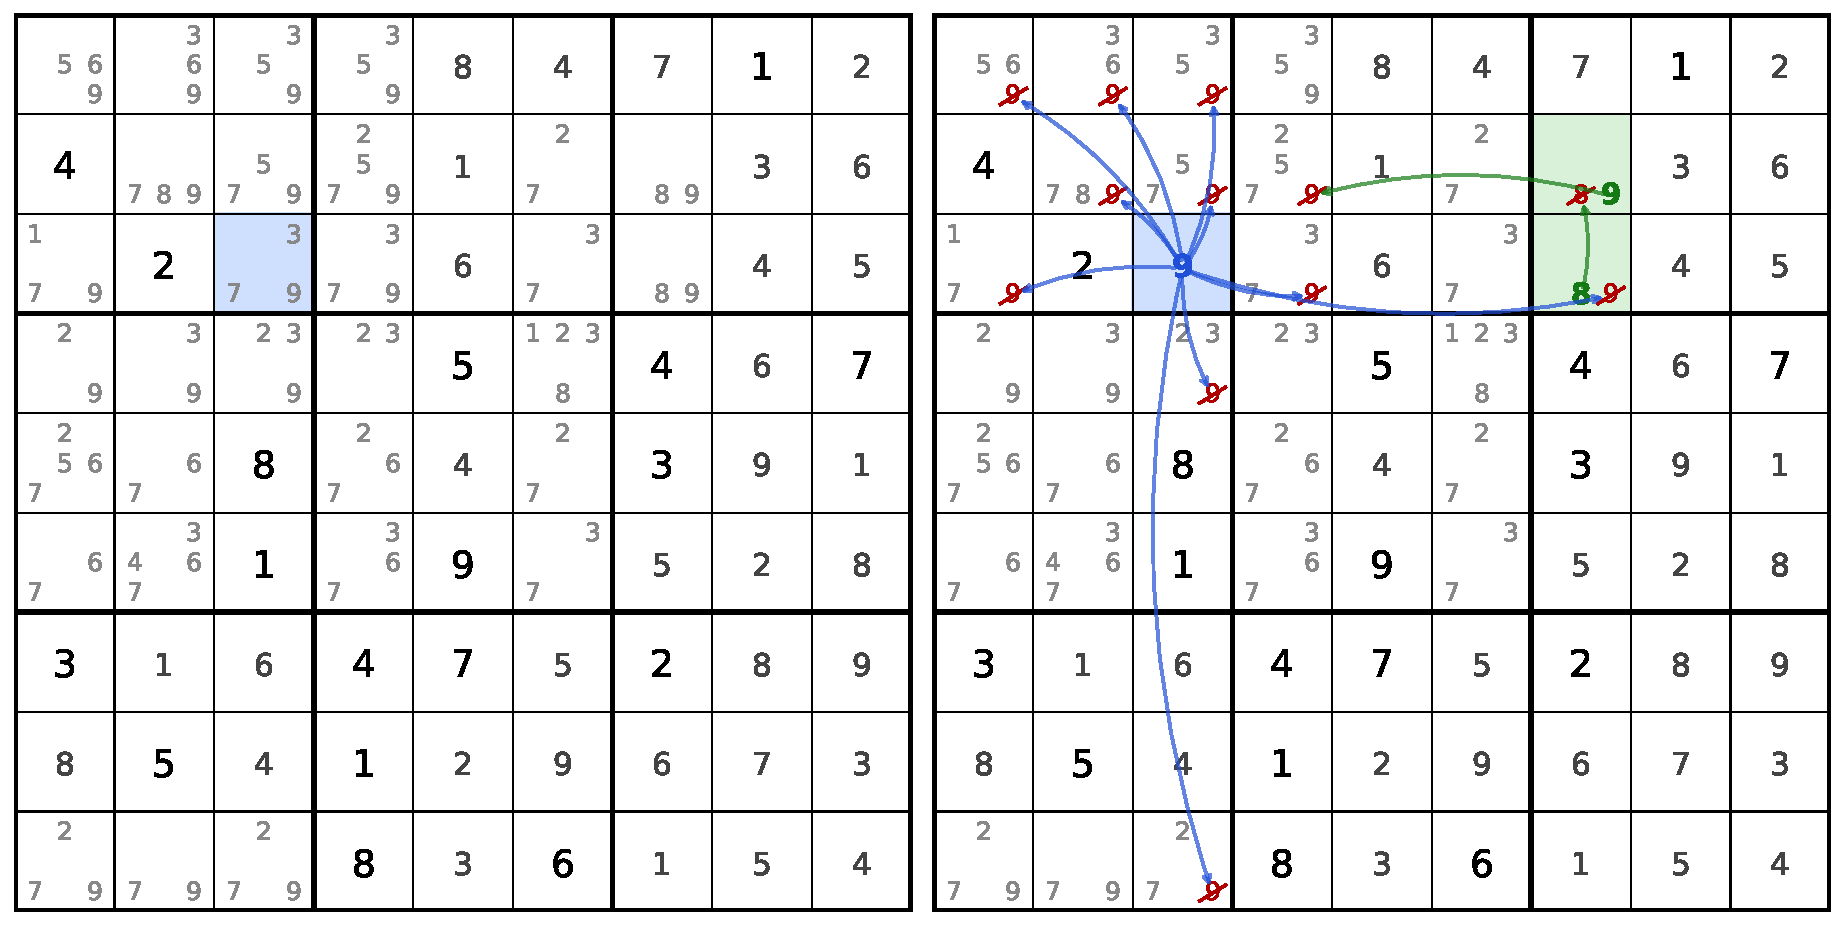
\includegraphics[width=\linewidth]{figures/sudoku/propagation_sudoku.pdf}
\caption{\textbf{Propagation} on a Sudoku: each cell is a variable, the
\emph{all-different} constraints on rows, columns, and boxes are the propagators,
and the small pencil marks are each cell's remaining candidates. \textbf{Left:}
the givens propagated as far as they go; every empty cell still has several
candidates and none is forced, so search must guess. \textbf{Right:} we guess a
\textbf{blue} value; the propagators strike it from every peer (blue arrows), one
peer loses its last alternative and is forced, which forces a \textbf{green}
value, and the deductions cascade to a new fixed point with no further guessing.}
\label{fig:sudoku-propagation}
\end{figure}

\begin{figure}[tb]
\centering
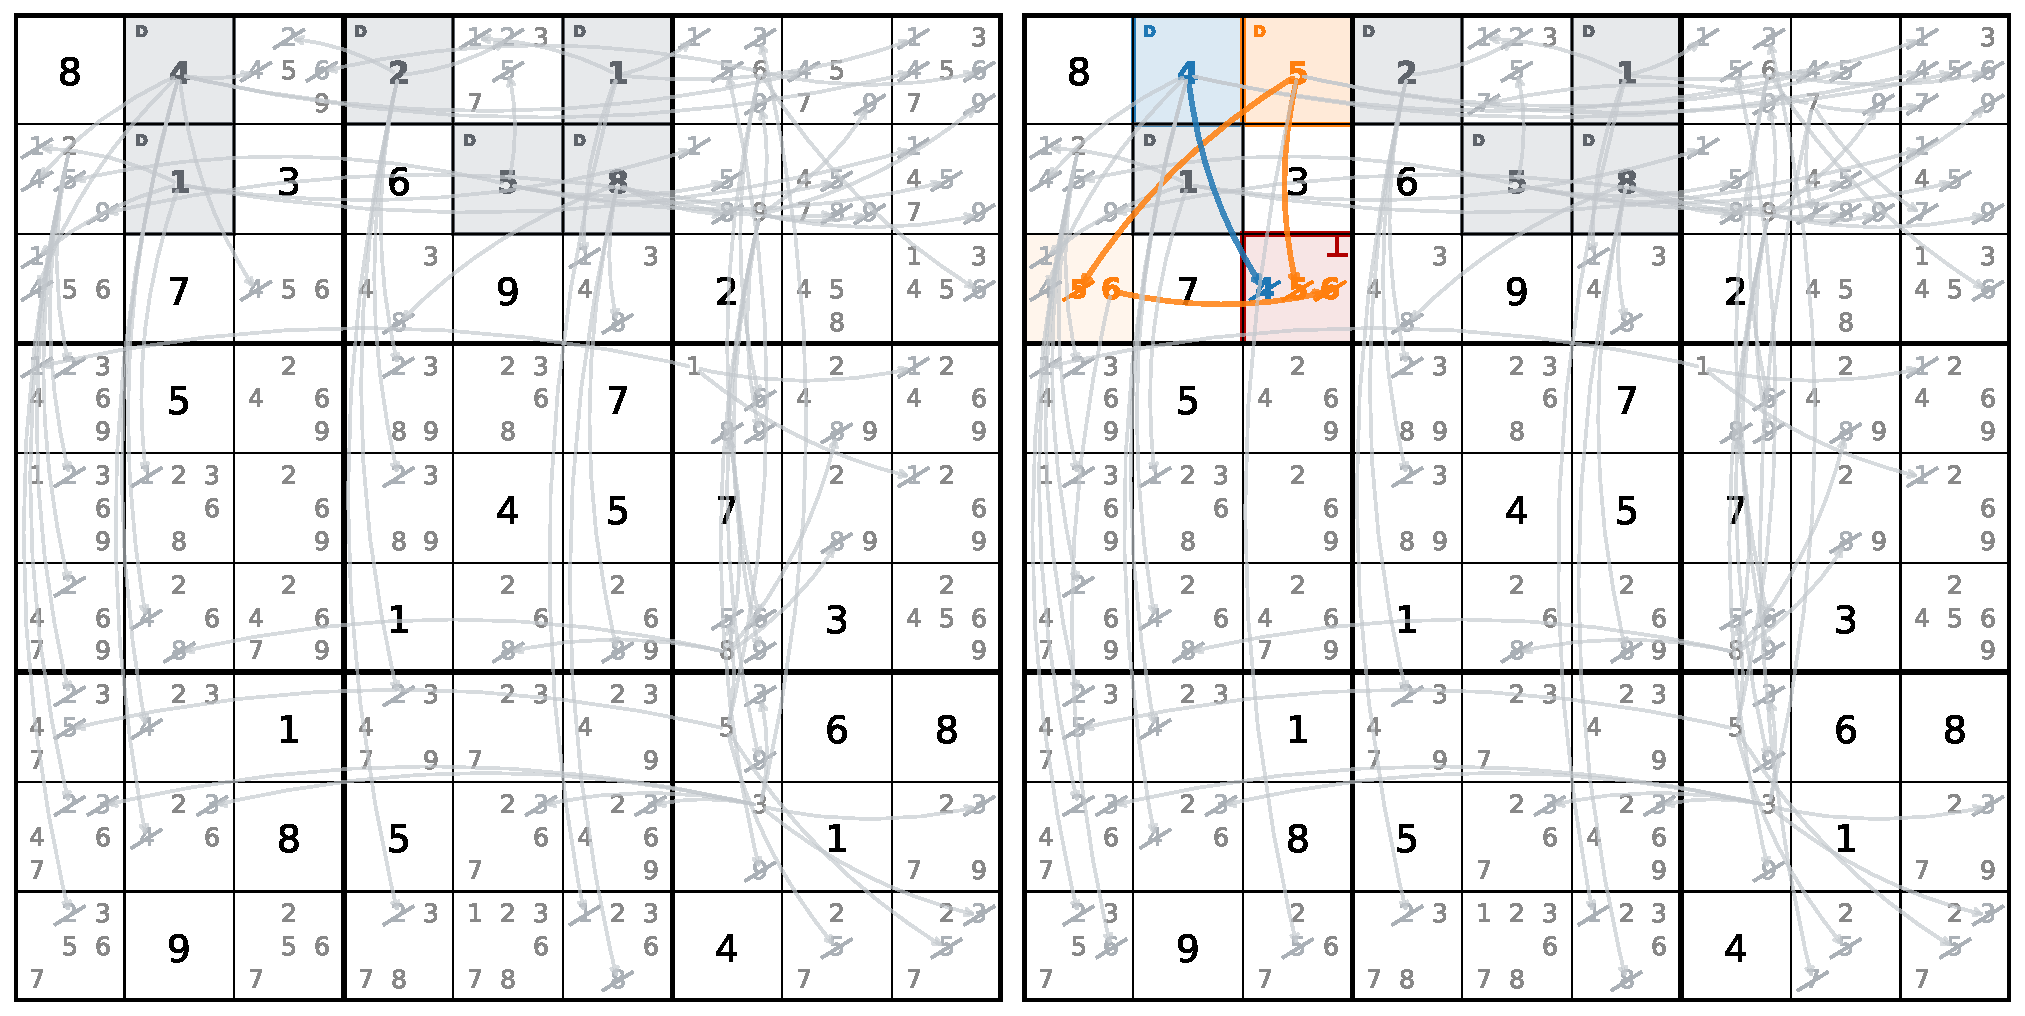
\includegraphics[width=\linewidth]{figures/sudoku/conflict_sudoku.pdf}
\caption{\textbf{Conflict analysis} on a Sudoku. \textbf{Left:} six guesses (grey,
tagged $D$) have been placed and propagated, and nothing has failed yet.
\textbf{Right:} a seventh guess (\textbf{orange}) propagates and empties one cell's
domain (\textbf{red}, $\bot$): a \textbf{conflict}. Tracing the struck candidates
backward shows that only \emph{two} of the seven guesses are jointly to blame (the
orange one and a \textbf{blue} one); the other five never touched this cell. From
these two the solver learns a \textbf{SAT clause} (a nogood) that bars the
combination forever, then backjumps past the five irrelevant guesses instead of
just undoing the last one.}
\label{fig:sudoku-conflict}
\end{figure}

Classic CP search is good at pruning but tends to be amnesiac: it backtracks and
forgets why it failed. Classic SAT learns effectively but only speaks in Boolean
clauses and cannot compactly express arithmetic relations among integer variables.
CP-SAT's central idea,
\textbf{lazy clause generation}, combines the two: CP-style propagators perform
the pruning, but every pruning step is justified by a reason from which the CDCL
engine can learn. The result is a CP solver with a SAT solver's memory.
% Source (developers' own framing of the lineage): the CP-SAT developers trace
% the architecture to Peter Stuckey's "Search is Dead" (CP 2013) and the lazy
% clause generation line of work, deliberately discarding classic CP search
% machinery in favor of a SAT core that learns.
\begin{platypusbook}[htb]
The developers trace CP-SAT's lineage directly to the lazy-clause-generation work of
the late 2000s, notably Peter Stuckey's pointed ``search is dead'' framing, and
built CP-SAT by deliberately discarding the classic CP search machinery in favor
of a learning SAT core. For the fuller story, see Stuckey's
\href{https://youtu.be/lxiCHRFNgno}{talk on lazy clause generation}~\cite{stuckey2014lcg}
and the CP-SAT developers' own overview talks~\cite{perron2020cpaior,perron2024scheduling,perron-ewo-ortools}.
\end{platypusbook}

Two further ingredients complete the picture. The rest of this text treats them
as accelerators bolted onto the core (\cref{part:faster}, \emph{Going faster}),
but they are central to what CP-SAT \emph{is}, and any honest description should
name them up front.

\begin{itemize}
  \item \textbf{A linear-programming relaxation, run as a propagator.} Alongside
  the search, LP-enabled CP-SAT workers maintain a continuous LP relaxation of
  the model and re-solve it with the dual simplex as a high-cost propagator,
  typically after cheaper propagation has stalled. The LP relaxation feeds back
  global numeric bounds, reduced-cost reasoning, and cutting planes
  (\cref{sec:lp,sec:cuts}). This creates the bridge to the
  \textbf{MIP} (mixed-integer programming) world of branch-and-cut: a third
  solver tradition folded in beside CP and SAT, and the reason CP-SAT holds its
  own on problems with strong linear structure where pure propagation is weak.
  \item \textbf{A parallel portfolio, not a single search.} Given several
  threads, CP-SAT does not partition one tree. It runs a \textbf{portfolio} of
  workers instead, most of them differently configured copies of the same core
  (some LP-heavy, some pure CP/SAT, some core-guided on the objective), together
  with a set of primal heuristics. These
  workers attack the whole problem at once and continuously share the clauses
  and bounds they learn (\cref{sec:portfolio}).
\end{itemize}

So the compact answer to ``what is CP-SAT?'' is: a CDCL learning core, fed by CP
propagation \emph{and} an LP relaxation, diversified across a cooperating
portfolio.

\section{Foundations}\label{part:foundations}

This section assembles the search core from its parts: the data model every other
piece reads and writes, the propagation that reasons over it, and the branching
that turns a pruned domain into a concrete solution. We start with how a variable
is stored, look inside a single propagator, sort out which high-level constraints
are expanded away versus kept as propagators, and finish with how search drives a
range down to one value.

\begin{platypusbook}[htb]
A working familiarity with CDCL SAT solving (decisions, unit propagation,
conflict analysis, clause learning, and backjumping) is not strictly required
here, but it is highly recommended. CP-SAT layers a good deal on top of a CDCL
core, so having seen how a plain CDCL solver works makes the rest considerably
easier to follow. Readers who want that background first can start with Smock's
gentle visual introduction
\cite{smock2016peek} (about 35 minutes), move on to Nadel's more technical talk
linking CDCL to optimization \cite{nadel2023cdcl}, and turn to Biere's in-depth
tutorial \cite{biere2021satsolving} (about four and a half hours) for the full
machinery. Knuth's fascicle \cite{knuth2015satisfiability} is the canonical
written reference, useful either in place of the videos or alongside them.
\end{platypusbook}

\subsection{The data model: variables as bounds}\label{sec:bounds}
% Sources (VERIFIED):
%   ortools/sat/integer_base.h -- IntegerLiteral (x >= bound / x <= bound),
%     GreaterOrEqual()/LowerOrEqual(); negation flips the bound.
%   ortools/sat/integer.h -- IntegerTrail stores monotone lower bounds
%     (upper bound = lower bound on NegationOf(var)); a var is fixed when lb==ub.

Everything that follows rests on a single design decision: \emph{how the solver
represents an integer variable while it is running}. Once this idea is clear,
the rest of the architecture (propagation, reasons, and learning) falls into
place almost inevitably.

\textbf{Variables are bounds, not values.} An integer variable $x$ with domain
$[0,10]$ is \emph{not} stored as a tentative value, such as ``$x$ is currently
$3$.'' It carries no working assignment at all: nothing like the fractional
value a MIP branch-and-bound node rounds, or the running guess a heuristic nudges
toward feasibility. Instead it is stored as a pair of \textbf{current bounds}, a
lower bound $\text{lb}(x)$ and an upper bound $\text{ub}(x)$. Search and
propagation never \emph{assign} $x$; they only \emph{narrow} the gap between these
two numbers, and $x$ is \emph{fixed} only once they meet.

This puts CP-SAT close to a classical finite-domain solver, which also narrows
rather than assigns, but with one decisive difference. A finite-domain solver
keeps the full set of surviving candidate values and lets a propagator strike any
one of them, every even number say, out of the interior of a domain. CP-SAT's
propagators move only the lower and upper bounds. The integer trail reasons about
$x$ through those two numbers alone, treating the live domain as the interval
$[\text{lb}(x), \text{ub}(x)]$ between them. When the declared domain has holes,
this interval is an \emph{over-approximation}: bound propagation works on the
enclosing interval, while the holes themselves are tracked separately, by presolve
canonicalization and the integer encoding of \cref{sec:encoding}. Until that
section, treat every domain as a plain interval.

As the solver descends the search tree, the bounds tighten ($\text{lb}$ rises and
$\text{ub}$ falls); when it backtracks, they relax again. Domains therefore shrink
from the outside in and grow back the same way.

Two properties of this representation make it work:

\begin{itemize}
  \item \textbf{Monotonicity.} Within one root-to-node path, the bounds only move
  inward. A propagator never has to reconcile competing updates; it only reads
  the tightest bounds known so far.
  \item \textbf{Reversibility.} Because a bound is a single number stamped with
  the decision level that set it, undoing work on backtrack is simple: pop every
  bound change made above the level to which the solver jumps. This integer
  trail, a stack of bound changes, is the same one that powers conflict analysis
  (\cref{sec:learning}).
\end{itemize}

\textbf{The atomic fact: a bound literal.} If variables are bounds, then the
elementary statements the solver asserts and reasons about are \textbf{bound
literals}: claims of the form
\[
  \bl{x \ge 5} \qquad\text{or}\qquad \bl{x \le 3} .
\]
The double brackets mark the claim as an \emph{object} the solver holds,
enqueues, and gathers into reasons, as opposed to the bare arithmetic relation
$x \ge 5$; we write them where that literal-as-object reading is what matters and
drop them in running prose where it is not. A bound literal is the integer analog
of a Boolean SAT literal, and, crucially, it behaves like one in the two ways the
learning machinery needs. (These are
exactly what the source calls an \srcla{integer\_base.h}{207}{IntegerLiteral}; this text says ``bound
literal'' throughout, but the two names refer to the same object.) It
\emph{negates cleanly}: over the integers, the negation of $x \ge 5$ is exactly
$x \le 4$. Moreover, a conjunction of bound literals describes an interval, so
the current domain $[\text{lb},\text{ub}]$ is just the two literals
$x \ge \text{lb}$ and $x \le \text{ub}$ held true at once. A variable is
\textbf{fixed} when its bounds meet, $\text{lb}(x) = \text{ub}(x)$: the interval
has collapsed to a single value, and this is the only sense in which $x$ ever
``has'' a value during search.

\textbf{Why this unifies the whole solver.} This representation lets a single
engine reason about a Boolean variable with domain $\{0,1\}$ and a wide integer
variable with domain $[0,10^6]$ through one common atom: the literal. A Boolean
assignment is already a literal, and an integer bound is a bound literal
$\bl{x \ge v}$ of the kind the previous paragraph introduced.
The two meet, but not because a Boolean is secretly an integer; it is the other
way around. When search needs to decide an integer bound, that bound is
\emph{reified}: turned into a Boolean literal (\cref{sec:encoding}) and handed to
the SAT core, which then drives the search on it: it can take that literal as a
decision, maintain its activity, and let learned clauses propagate it directly.
Deciding a Boolean and committing to an integer bound thus become the same kind
of step, recorded at \emph{one} shared decision level, which is precisely what
lets the SAT half and the CP half cooperate under \emph{one} conflict-analysis
mechanism rather than passing messages between two separate solvers.

\subsection{The trail}\label{sec:trail}
% Sources (VERIFIED):
%   ortools/sat/sat_base.h -- class Trail (331): the Boolean trail; AssignmentInfo
%     (277) stamps each entry with its decision level; EnqueueSearchDecision (425)
%     opens a new level for a decision; Reason() (525) returns a forced literal's
%     reason; Untrail() (595) truncates the trail on backjump.
%   ortools/sat/integer.h -- class IntegerTrail (523): the integer trail; Enqueue()
%     (745) pushes a bound change; integer_trail_ (1123) is the stack of bound
%     entries; Untrail() (547) unwinds it in lockstep with the Boolean trail.

A solver that guesses and backtracks needs a precise record of what it has
assumed and what followed. That record is the \textbf{trail}
(\srcla{sat\_base.h}{331}{Trail}): the ordered, append-only log of every literal
asserted on the current path from the root of the search tree to the node being
explored. Two kinds of entry land on it: \emph{decisions}, the literals the
solver guesses (\srcla{sat\_base.h}{425}{EnqueueSearchDecision} and
\cref{sec:complete}), and the literals propagation then forces from them.
Each entry is stamped with the \textbf{decision level} at which it was added
(\srcl{sat\_base.h}{277}), and each forced entry also carries a \emph{reason}
(\srcl{sat\_base.h}{525}), the facts that entailed it (\cref{sec:learning}).
Backtracking to level $k$ truncates the trail to its level-$k$ prefix
(\srcla{sat\_base.h}{595}{Untrail}), undoing every later assertion in one
step. The trail is thus both the solver's working memory and the substrate
conflict analysis walks backward when a guess fails.

CP-SAT reasons in two kinds of literal, so it keeps two coupled trails. Bound
changes accumulate on the \textbf{integer trail}
(\srcla{integer.h}{523}{IntegerTrail}, the stack \srcla{integer.h}{1123}{integer\_trail\_}), the stack of bound literals introduced above; Boolean
assignments accumulate on the \textbf{Boolean trail}. The two are not
independent: they share one decision-level counter, so they advance and unwind
together (the integer trail's \srcla{integer.h}{547}{Untrail} fires with
the Boolean one), and a bound the solver has reified into a Boolean is recorded
on both. An ordinary propagated bound, by contrast, lives only on the integer
trail. Keeping bound changes on a native integer trail, rather than as Booleans,
is what makes the encoding of \cref{sec:encoding} lazy: most bound movements
never touch the Boolean trail at all. Where this text says \emph{the} trail, it
means the single timeline the two structures form together.

\subsection{Propagation: the CP half}
% Sources (VERIFIED):
%   ortools/sat/integer.h -- PropagatorInterface (Propagate()/IncrementalPropagate());
%     GenericLiteralWatcher schedules registered propagators to a fixed point
%     (WatchLiteral/WatchLowerBound/WatchUpperBound, Register()).
%   Global constraints live in ortools/sat/ (e.g. all_different.*, no_overlap*/
%     scheduling*, circuit.*, cumulative.*, diffn.*).

With variables reduced to bounds, we can say precisely what a constraint
\emph{does} during search: it narrows those bounds. Each constraint comes with a
\textbf{propagator}, a piece of reasoning that, given the current bounds of the
variables it touches, tightens those bounds or reports a conflict when no value
remains.

Consider a simple example:
\[
  x \in [0, 10],\quad y \in [0, 10],\quad z \in [0, 10],
  \qquad \text{constraint: } x + y \le z .
\]
If, at some point, $z \le 4$ and $y \ge 2$, the linear propagator deduces
$x \le 2$ and pushes this new bound onto the trail. That deduction may wake
another propagator watching $x$, which may tighten another bound, and so on.
Propagators fire in cascade until the system reaches a \textbf{fixed point}: no
propagator can deduce anything new. Alternatively, one of them may detect a
\textbf{conflict}; for example, it may need $x \le 2$ while the trail already
contains $x \ge 3$, leaving the domain of $x$ empty.

Global constraints such as
\srcla{all\_different.h}{52}{AllDifferent}, \srcla{disjunctive.h}{49}{NoOverlap} (scheduling), \srcla{circuit.h}{46}{Circuit} (routing),
and \srcla{cumulative.h}{48}{Cumulative} (resources) carry specialized algorithms that prune far
more aggressively than a collection of generic inequalities could. Yet however
hard it prunes, \textbf{propagation alone never makes a choice}: everything it
concludes is a forced consequence of the current bounds. When it runs out of
necessary conclusions and the problem is not yet solved, search must guess.

\Cref{fig:sudoku-propagation} shows this guess-and-cascade on a Sudoku. One caveat
carries through the rest of this text: CP-SAT does \emph{not} carry hole-punched
domains like the pencil marks in that figure. It propagates only each variable's
lower and upper \emph{bounds} and hands every interior elimination to the SAT
engine as a Boolean literal. The bound-literal form of exactly this reasoning is
the implication graph in \Cref{fig:uipgraph}.

\subsection{Example: a propagator for $3x + 6y \le z$}\label{sec:onepropagator}
% Sources (VERIFIED):
%   ortools/sat/integer_expr.h:71-169 -- class LinearConstraintPropagator<use_int128>
%     : public PropagatorInterface, LazyReasonInterface; aliases IntegerSumLE /
%     IntegerSumLE128. Constraint stored canonically as sum_i coeff_i*var_i <= ub
%     (positive coeffs; a variable on the "other side" enters as NegationOf(var)).
%   integer_expr.cc:444-458 -- RegisterWith(): WatchLowerBound(vars_[i], id) for
%     every variable -> woken incrementally only when a watched LOWER bound moves.
%   integer_expr.cc:300-311 -- slack = ub - sum_i coeff_i*lb(var_i).
%   integer_expr.cc:334-368 -- Propagate(): for each i pushes new_ub_i = lb_i +
%     floor(slack/coeff_i) via EnqueueWithLazyReason(LowerOrEqual(var_i,new_ub),
%     0, propagation_slack, this).
%   integer_expr.cc:228-233 -- Explain() (LazyReasonInterface) returns ONLY the
%     raw reason: boolean_literals_at_false + vars_ + coeffs_ (ALL variables).
%     It does NOT read the slack, does NOT drop the explained var, does NOT relax.
%     (Args id/to_explain are unused in the body.)
%   integer.h:1145 LazyReasonEntry::Explain -- the TRAIL sets reason->slack =
%     propagation_slack (stored at EnqueueWithLazyReason time), then calls the
%     propagator's Explain().
%   integer.cc:1956-2022 ComputeLazyReasonIfNeeded -- the TRAIL drops the
%     propagated var (to_ignore) and, if slack>0, calls RelaxLinearReason(
%     reason->slack, coeffs, indices) at integer.cc:2021. THIS is where the
%     stored slack is consumed for an ordinary push.
%   integer_expr.cc:110-121 -- FillIntegerReason(): collects the bounds used.
%   integer_expr.cc:299-327 -- CONFLICT path only (slack<0): the propagator
%     itself calls RelaxLinearReason(-slack-1,...) at :314 + ReportConflict() at
%     :325 (or EnqueueLiteral when a single enforcement literal is unassigned).

In the CP-SAT source a propagator is wrapped in templates, watch lists, and
lazy-reason plumbing, but the object underneath is small. As a worked example, consider the linear propagator for $3x + 6y \le z$ over
$x, y \in [0,3]$ and $z \in [0,30]$, following what CP-SAT's
\srcla{integer\_expr.h}{72}{LinearConstraintPropagator} actually does. CP-SAT stores
every linear constraint in \emph{canonical form}, all terms on one side of a
constant, so throughout we work with it as
\[
  3x + 6y - z \le 0 ,
\]
where the term $-z$ is the variable $\srcla{integer\_base.h}{175}{NegationOf}(z)$.
The role comes with two duties. In a classical finite-domain
solver a propagator has only the first: narrow domains, then say no more. A
CP-SAT propagator must also \emph{justify} each deduction on demand, naming the
bounds that forced it, so that the learning half (\cref{sec:learning}) can
distill a failure into a permanent rule. That second duty, explaining a
propagation rather than merely performing it, is what \emph{lazy clause
generation} adds to ordinary propagation; it is the one a classical propagator
does not carry.

\textbf{We are called only when a watched bound changes.} Running the propagator on
every change in the search would be wasteful; we want it to fire only when something
has happened that could let us deduce more. So on creation we register with the
\srcla{integer.h}{1324}{GenericLiteralWatcher}, asking to be called whenever the
\emph{lower} bound of $x$, $y$, or $-z$ changes (\srcla{integer\_expr.cc}{449}{WatchLowerBound} on each); we are never run on a step that touched none of the
three. For a ``$\le$'' constraint only the lower bounds matter: they are what can
push the left-hand side up toward the bound. Because $z$ enters as $-z$, the update
``$z$'s upper bound fell to $8$'' reaches us as ``the lower bound of $-z$ rose to
$-8$,'' so a single watch direction already covers both sides of every variable,
directly reflecting the bounds-as-everything data model of \cref{sec:bounds}.

\textbf{If the constraint is violated, we report a conflict.} Whenever a watched
bound moves, we recompute our \emph{slack}, the room left before the constraint
binds (\srcl{integer\_expr.cc}{310}):
\[
  \text{slack} \;=\; \underbrace{0}_{\text{rhs}}
  \;-\; \big(3\,\text{lb}(x) + 6\,\text{lb}(y) + 1\cdot\text{lb}(-z)\big) .
\]
If it is negative, the current bounds already rule the constraint out and there is
nothing to deduce: we report a conflict. Suppose decisions have forced $x \ge 2$
and $y \ge 1$ while $z \le 8$, so $\text{lb}(x) = 2$, $\text{lb}(y) = 1$, and
$\text{lb}(-z) = -8$; then
\[
  \text{slack} \;=\; 0 - (3\cdot 2 + 6\cdot 1 + 1\cdot(-8)) \;=\; -4 \;<\; 0
\]
(\srcl{integer\_expr.cc}{312}). We do not backtrack or learn; that is the SAT
half's job. We simply fill our reason $\{x \ge 2,\ y \ge 1,\ z \le 8\}$ and call
\srcla{integer\_expr.cc}{325}{ReportConflict}, declaring that these bounds
are jointly impossible. The conflict analysis of \cref{sec:learning}
takes it from there.

\textbf{What we read, and what we push.} When the slack is non-negative there is
room to spare, and instead of failing we tighten bounds. Take the lighter state
where $x$ and $y$ still sit at their lower bound $0$ while $z \le 8$, so the slack
is $0 - (3\cdot 0 + 6\cdot 0 + 1\cdot(-8)) = 8$.
This is not a conflict, but we could already prove that $x \le 2$ and $y \le 1$ must hold, since any higher would push the left-hand side above $8$.
Reading only the \emph{lower} bounds of the other
variables, we push an \emph{upper} bound on each variable
(\srcl{integer\_expr.cc}{334}):
\[
  \text{new\_ub}_i =
  \text{lb}_i + \left\lfloor \frac{\text{slack}}{\text{coeff}_i} \right\rfloor .
\]
For this example, the resulting bounds are
\[
  x \le 0 + \lfloor 8/3 \rfloor = 2, \qquad\qquad
  y \le 0 + \lfloor 8/6 \rfloor = 1 .
\]
Both tighten the domain: $x$ shrinks from $[0,3]$ to $[0,2]$, and $y$ shrinks
from $[0,3]$ to $[0,1]$. That is the whole job: read the other variables' bounds
and push tighter bounds of our own. There is no guessing and no search, only
forced consequences.
% Source (VERIFIED): template LinearConstraintPropagator<use_int128> and the alias
%   IntegerSumLE128 (integer_expr.h:71,168-169); int128 activity/slack at
%   integer_expr.cc:258-310 ("absl::int128 lb_128 = 0;", "slack128 = int128(ub) - lb_128").
\begin{platypusinfo}[htb]
When a constraint's coefficients and bounds are large enough that the running
activity could overflow $64$ bits, CP-SAT instantiates the linear-sum propagator
in a $128$-bit variant (\srcla{integer\_expr.h}{169}{IntegerSumLE128}): the
coefficients remain \code{int64}, but activity and slack accumulate in
\code{int128}. The bound it pushes is therefore the exact integer bound, not a
wrapped-around value: the solver keeps its arithmetic exact all the way down to a
single linear row.
\end{platypusinfo}

\textbf{Why do we not directly add these insights as clauses?}
In principle we could add a clause for the implication
\[
  (\bl{x \ge 0} \;\wedge\; \bl{z \le 8}) \;\Rightarrow\; \bl{y \le 1}
\]
outright, but that is both costly and unnecessary. For now it is enough to tell the
search that $y \le 1$, which updates the bounds and may wake other propagators; we
owe an explanation only if $\bl{y \le 1}$ later turns out to be part of a conflict, when
conflict analysis needs the deduction to trace the root cause and learn a clause.
And the more precise that reason, the more effective the learning: here it is
trivial, but for a constraint over many variables it can pay to do real work at
explain time and pinpoint exactly the subset of bounds that forced the deduction.
CP-SAT's \srcla{cp\_constraints.cc}{123}{GreaterThanAtLeastOneOf} propagator does
exactly this: its \code{Explain} drops the bounds already implied at the root and
returns that trimmed subset rather than the whole row. Since most deductions never
enter a conflict at all (look at how few bounds the conflict in
\cref{fig:sudoku-conflict} actually rests on), computing and storing a precise
reason for every one of them would be wasted effort.

\textbf{So how is the reason attached?} Rather than record the justification, we
call \srcla{integer\_expr.cc}{360}{EnqueueWithLazyReason} and hand the trail
only a pointer back to ourselves. The trail enqueues $y \le 1$ and wakes whatever
that unblocks, but stores no explanation alongside it. Only if this deduction is
later dragged into a conflict does the engine call our \srcla{integer\_expr.cc}{228}{Explain} method; only then do we name the bounds that forced the push,
$x \ge 0$ and $z \le 8$, handing back the implication above for conflict analysis
(\cref{sec:learning}) to resolve and learn from. The reason is available the
whole time, but built only for the deductions that turn out to need it. This is lazy
clause generation at the scale of a single propagator.

At its core, the entire object consists of two short
procedures: one that pushes bounds and one that explains them on request. The
trail owns the events, the propagator only responds, and the explanation is a
deferred call-back that the trail makes only if a pushed bound is later dragged
into a conflict.

\begin{algorithm}[htbp]
\caption{Linear propagator for $\sum_i c_i x_i \le u$ in canonical form (all $c_i > 0$)}
\label{alg:linprop}
\begin{algorithmic}[1]
\Procedure{Propagate}{} \Comment{woken when a watched lower bound rises}
  \State $\text{slack} \gets u - \sum_i c_i \cdot \text{lb}(x_i)$ \Comment{room before the constraint binds}
  \If{$\text{slack} < 0$}
    \State \Return \Call{ReportConflict}{$\{\, \bl{x_i \ge \text{lb}(x_i)} \,\}_i$} \Comment{bounds jointly impossible}
  \EndIf
  \ForAll{$i$}
    \State $\text{newub} \gets \text{lb}(x_i) + \lfloor \text{slack}/c_i \rfloor$
    \If{$\text{newub} < \text{ub}(x_i)$}
      \State \Call{EnqueueWithLazyReason}{$\bl{x_i \le \text{newub}}$, \ \textbf{self}}
    \EndIf
  \EndFor
\EndProcedure
\Statex
\Procedure{Explain}{$\bl{x_j \le v}$} \Comment{called \emph{only} if this pushed bound enters a conflict}
  \State \Return $\{\, \bl{x_i \ge \text{lb}(x_i)} \,\}_i$ \Comment{the raw reason: \emph{all} variables, unrelaxed}
\EndProcedure
\end{algorithmic}
\end{algorithm}

\subsection{Lifting the reason}\label{sec:relaxation}

We kept the propagator deliberately simple: its \code{Explain} hands back the raw
row, the full set of bounds that were in force, without hunting for the smallest or
most general subset. CP-SAT makes up for that afterward. Conflict analysis
(\cref{sec:learning}) turns each reason into a permanent clause, and a
\emph{weaker} reason, one that holds in more states, becomes a clause that rules out
more of them. So before learning, CP-SAT \emph{lifts} the reason
(\srcla{integer.cc}{1083}{RelaxLinearReason}): it spends the slack the deduction
left unused to loosen the bounds, recovering a more general clause than the
propagator literally reported.

Why is this sound? Because a push rarely uses all the room it had. Take the push of
$y \le 1$, made when the slack was $8$; reading off $\lfloor 8/6 \rfloor = 1$ gave
$y \le 1$, but the leftover
\[
  \ell \;=\; \big(\lfloor 8/6 \rfloor + 1\big)\cdot 6 \;-\; 8 \;-\; 1
        \;=\; 2\cdot 6 - 8 - 1 \;=\; 3
\]
measures how much room was to spare. Forcing $y \le 1$ never needed the full bound
$z \le 8$: even $z \le 11$ leaves $y \ge 2$ impossible once $x \ge 0$ is known,
since $3\cdot 0 + 6\cdot 2 = 12 > 11$. So CP-SAT lifts $z \le 8$ to $z \le 11$,
weakening the bound by exactly $\ell = 3$, and conflict analysis resolves against
the broader implication
\[
  (x \ge 0 \;\wedge\; z \le 11) \;\Rightarrow\; y \le 1
\]
instead of the tighter $z \le 8$ form, learning a clause that can fire in more
future states. The same trick broadens reported conflicts: there the slack is
already negative, and its magnitude is the budget for loosening the bounds the
violation did not strictly need.

All the propagator had to store to make this possible was a single integer, the
leftover slack, carried alongside its claim check rather than a copied reason. That
one number is what lets CP-SAT recover not merely \emph{a} reason but a deliberately
general one.

\subsection{Expansion: which constraints keep a propagator}\label{sec:expansion}
% Sources (VERIFIED):
%   ortools/sat/cp_model_expand.cc -- ExpandElement (1159), ExpandPositiveTable
%     (2288)/ExpandNegativeTable (1673), ExpandAutomaton (1318), ExpandInverse (679),
%     MaybeExpandAllDiff (2713, heuristic: small / near-permutation / fully encoded),
%     ExpandReservoir (406, default-ON via expand_reservoir_constraints=true),
%     ExpandLinMax (808, size-gated; max_lin_max_size_for_expansion default 0 = kept). Default behavior
%     KEEPS native propagators; expansion is heuristic / parameter-gated.
%   ortools/sat/cp_model_loader.cc -- kept propagators are loaded here:
%     LoadBoolOr/BoolAnd/BoolXor (clauses), LoadLinearConstraint (1213, supports
%     enforcement literals = half-reification), LoadAllDiffConstraint -> AllDifferentOnBounds
%     (1485), LoadCircuit/Routes (1664/1679), LoadNoOverlap/Cumulative/NoOverlap2d
%     (1610/1629/1616), LoadIntProd/IntDiv/FixedModulo (1506/1553/1576).
%   VISIBLE LINKS for kept constraints point past the one-line loader to the
%     algorithm header where the propagator/factory + its doc comment live
%     (re-verify these line numbers when re-pinning \orsha):
%       AllDifferent (kept "on bounds") -> all_different.h:52 (AllDifferentOnBounds)
%       NoOverlap    -> disjunctive.h:49 (AddDisjunctive)
%       NoOverlap2d  -> diffn.h:89 (AddNonOverlappingRectangles)
%       Cumulative   -> cumulative.h:48 (Cumulative)
%       Circuit      -> circuit.h:46 (class CircuitPropagator)
%       MultipleCircuit -> circuit.h:259 (LoadSubcircuitConstraint, wraps CircuitPropagator)
%     The heuristically-expanded AllDifferent mention still links MaybeExpandAllDiff
%     (cp_model_expand.cc:2713); the Expanded-away names keep their Expand* targets.

\cref{sec:onepropagator} said that every constraint type has a
propagator. That is only half the story. A modeling language offers dozens of
high-level constraints, and CP-SAT does \emph{not} keep a bespoke propagator for
each of them. During presolve, many constraints are \textbf{expanded}: rewritten
into the small set of primitives that the engine reasons about natively, such
as clauses, linear constraints, at-most-one constraints, and value literals.
Only a curated subset is \textbf{kept} as dedicated global propagators.

\textbf{Expanded away} (\srcf{cp\_model\_expand.cc}):
\srcla{cp\_model\_expand.cc}{1159}{Element},
\srcla{cp\_model\_expand.cc}{2288}{Table} (positive and negative),
\srcla{cp\_model\_expand.cc}{1318}{Automaton}/regular, and
\srcla{cp\_model\_expand.cc}{679}{Inverse}. CP-SAT may also expand
\srcla{cp\_model\_expand.cc}{2713}{AllDifferent} heuristically when its domain
is small or close to a permutation; in that case, it becomes value literals plus
at-most-one constraints. Two more sit on a parameter-controlled line:
\srcla{cp\_model\_expand.cc}{406}{Reservoir} is expanded \emph{by default} (a
parameter can instead keep it native), while
\srcla{cp\_model\_expand.cc}{808}{LinMax} constraints keep their propagator
\emph{by default}, with a size threshold that opts only the \emph{small} ones into
expansion.
% LinMax gating (cp_model_expand.cc:2875): expand iff exprs().size() <=
%   max_lin_max_size_for_expansion, default 0 (sat_parameters.proto:578) -> nothing
%   expanded unless the threshold is raised, and then it is the SMALL constraints that
%   get expanded, not the large ones. Prose previously said "large ... unless a size
%   threshold opts them into expansion", which points the mechanism at the wrong end.
The common thread is not
that a stronger native propagator could never exist; it is that the decomposition
is often cheap, exposes useful Boolean or value structure to the rest of the
engine, or is competitive enough that a dedicated algorithm would not reliably
pay for itself.

\textbf{Kept as native propagators} (\srcf{cp\_model\_loader.cc}): Boolean
constraints, loaded as clauses; \textbf{linear} constraints, crucially
\emph{with enforcement literals}, that is, half-reified ``indicator'' constraints
in which a literal $\ell$ enforces a linear constraint; integer \textbf{product}
(variable~$\times$~variable), \textbf{division} (the divisor may be a variable),
and \textbf{modulo} constraints (the modulus must be a fixed constant; a variable
modulus is decomposed into division and product during presolve);
% int_prod/int_div/int_mod loaded natively in cp_model_loader.cc (VERIFIED):
%   LoadIntProd (1506) -> ProductConstraint (integer_expr.h:793); fully general var x var.
%   LoadIntDiv  (1553): denom fixed -> FixedDivisionConstraint (integer_expr.h:836),
%     ELSE DivisionConstraint (integer_expr.h:817). A variable divisor IS native --
%     so "fixed divisors" was wrong for division (and meaningless for product).
%   LoadIntMod  (1576): CHECK(IsFixed(mod)) -> FixedModuloConstraint (integer_expr.h:851);
%     there is no variable-modulus propagator. ExpandIntMod (cp_model_expand.cc:575)
%     rewrites a non-fixed modulus into int_div + int_prod + linear during presolve.
\srcla{all\_different.h}{52}{AllDifferent} on bounds when it is \emph{not} a
small permutation; \srcla{circuit.h}{46}{Circuit} and
\srcla{circuit.h}{259}{MultipleCircuit} for routing; and the scheduling trio
\srcla{disjunctive.h}{49}{NoOverlap}, \srcla{cumulative.h}{48}{Cumulative}, and
\srcla{diffn.h}{89}{NoOverlap2d}. These are the constraints whose specialized
algorithms (edge-finding, energetic reasoning, subtour elimination, and
Hall-interval pruning) can prune far more than any clause decomposition could.
This is where the ``CP'' in CP-SAT does its real work.

This point is easy to oversimplify, so one nuance is worth stating plainly: the
released code \emph{defaults to keeping} native propagators, and expansion is
gated by size heuristics and parameters rather than applied wholesale. The
reason ties directly back to the cost argument of this part. A dedicated global
propagator is expensive, so CP-SAT keeps it only where its extra pruning tends
to pay for itself; everything else is handed to the cheap, always-on clause and
linear machinery.
\subsection{Search: guessing when propagation stalls}\label{sec:complete}
% Sources (VERIFIED):
%   ortools/sat/integer_search.h -- BooleanOrIntegerLiteral (a decision is a
%     Boolean OR an integer bound literal).
%   ortools/sat/sat_solver.cc -- EnqueueDecisionAndBackjumpOnConflict (binary
%     decisions, backjump on conflict). Heuristic detail moved to sec:search.

Whether a constraint reasons through a native propagator or an expanded
decomposition, propagation eventually runs dry: it reaches a fixed point with
nothing left to deduce. If every variable happens to be fixed, that fixed point
is a solution. Usually it is not. With no conflict, the fixed point may still
leave $3 \le x \le 7$ open: if every constraint is satisfiable across that whole
range, no propagator has any reason to tighten it. That is a consistent
\emph{state}, but not a \emph{solution}. A solution must assign $x$ one concrete
value, and propagation alone, which only ever draws forced conclusions, cannot
supply it. Closing the gap falls to \emph{search}.

The solver's only move at a stalled fixed point is to \emph{guess}. The guess is
a \textbf{decision}: it asserts a single literal, for instance trying
$\bl{x \le 7}$ true, with its negation $\bl{x \ge 8}$ held in reserve as the other branch. As \cref{sec:bounds}
noted, an integer bound is itself a reified literal, so guessing
$\bl{x \le 7}$ and flipping a native Boolean are the same step,
both recorded at a new \textbf{decision level}.

A decision sets off a fresh cascade of propagation, and the guess is judged by
what that cascade returns: it may pin more variables and let the solver descend
with another guess; it may fix everything with no conflict, giving a solution; or
it may reach a conflict, proving the guess wrong and forcing the solver to
\emph{backtrack} and learn (\cref{sec:learning}). Decisions stack on the
\textbf{trail}, each tagged with its decision level, and backtracking pops them
off and relaxes the bounds they imposed. Search is then just this loop: guess a
literal, let the resulting cascade say whether it was right, wrong, or simply not
yet decisive, and guess again until every variable is pinned. \emph{How} the
solver picks each literal, and what it does once the Booleans are all assigned
but an integer still spans a range, is the search machinery assembled in
\cref{sec:search}.

\section{Learning from failure}\label{part:learning}

Every propagator in \cref{part:foundations} can already report \emph{why} it made
each deduction: the reason behind each pushed bound. So far that capability has
gone unused, ready on every push but never once invoked. This section is
where it pays off. When propagation hits a dead end, those reasons let the solver
dissect the failure, trace it back to the handful of decisions truly responsible,
and distill that into a permanent rule, a single cheap clause, it never violates
again. That is the
faculty separating CP-SAT from classical CP, and the SAT half of the solver:
turning a single failure into knowledge instead of undoing it and forgetting.

\subsection{Conflict analysis and learning: the SAT half}\label{sec:learning}
% Sources (VERIFIED):
%   ortools/sat/integer.h -- IntegerTrail::Enqueue(i_lit, literal_reason,
%     integer_reason): every pushed bound carries a reason (false literals +
%     true integer literals); EnqueueWithLazyReason + LazyReasonInterface::Explain
%     for deferred (lazy) reasons.
%   ortools/sat/sat_solver.cc -- 1-UIP analysis, learned-clause + backjump
%     (detailed in the "worked conflict-analysis trace" section).

This is where CP-SAT departs from textbook CP, and where lazy clause generation
lives. When propagation derives a conflict, a plain CP solver would simply undo
the last decision and try the other branch. CP-SAT instead asks \textbf{why} the
failure happened, performing \textbf{conflict analysis}.

The mechanism that makes this possible is that every bound a propagator pushes
comes with a \textbf{reason}: the set of facts that forced it. When the
$x + y \le z$ propagator deduced $x \le 2$, its reason was ``$z \le 4$
and $y \ge 2$.'' A reason is, in essence, an implication:
\[
  (z \le 4 \;\wedge\; y \ge 2) \;\Rightarrow\; x \le 2 .
\]

These implications chain. When a conflict surfaces, the solver walks backward
through the reasons of the bounds involved, resolving them together until it
isolates a compact subset of decisions that is jointly responsible. From that
subset it builds a \textbf{learned clause}: a nogood that says, in effect,
``never again let all of \emph{these} conditions hold simultaneously.''

Three consequences follow, all inherited from CDCL SAT:

\begin{itemize}
  \item \textbf{The learned nogood is persistent} until it is deemed unhelpful
  and garbage-collected. It prunes not just this branch, but every future branch
  where the same combination would recur, possibly in a completely different
  part of the search tree.
  \item \textbf{Backjumping replaces chronological backtracking.} Conflict
  analysis identifies the \emph{real} culprit decision level, which may be far
  above the current one. The solver jumps straight back there in one step,
  undoing the intervening decisions and their propagations wholesale rather than
  retrying them level by level. This is far more powerful than the
  one-level-at-a-time backtracking of classical CP.
  \item \textbf{The learned clause itself propagates.} After backjumping, the
  new nogood immediately forces a bound, redirecting search productively instead
  of merely retrying.
\end{itemize}

The phrase \textbf{``lazy clause generation''} captures the efficiency trick
underneath: the implications justifying each deduction are \emph{not} eagerly
written out as stored Boolean clauses. A propagator's reason is assembled on the
spot when conflict analysis asks for it, resolved into the learned clause, and
otherwise left implicit. The overwhelming majority of deductions are made, used,
and undone on backtracking without any clause ever materializing; the solver pays
that cost only for the facts that turn out to matter for learning. Carrying
reasons is what makes this \emph{correct}: a learned clause is sound only because
its literals are exactly the facts that forced the conflict.

\Cref{fig:sudoku-conflict} shows this on a Sudoku: a single guess empties one
cell's domain, and walking the eliminations backward pins the blame on only two of
the seven guesses, so the solver learns a nogood over those two and backjumps past
the rest. The worked trace below makes the same steps precise on an integer model,
where each struck candidate becomes a Boolean bound literal.

\subsection{A worked conflict-analysis trace}\label{sec:trace}
% Sources (VERIFIED) -- the algorithm; the concrete linear example is illustrative
% (C0: x6>=x1+x2; C1: x4>=x3+1; C2: x5>=x4+x2; C3: x4+x5<=9; decisions x2>=2 @1,
%  x1>=3 @2 [fires C0: x6>=5, off-path], x3>=4 @3; level-3 cascade x4>=5, x5<=4
%  (C3), x5<=5 (order-enc link x5<=4 => x5<=5), x5>=7 (C2) => empty domain on x5
%  via threshold [x5>=6]; 1-UIP = x4>=5; learned {~[x4>=5], ~[x2>=2]};
%  assertion level 1 => non-chronological backjump over x1>=3 @2; hand-checked):
%   ortools/sat/sat_solver.cc -- ComputeFirstUIPConflict() (resolve failing
%     clause against reasons by decreasing trail index until one current-level
%     literal remains = UIP); ComputePropagationLevel() (assertion = 2nd-highest
%     level); AddLearnedClauseAndEnqueueUnitPropagation(); ComputeLbd();
%     MinimizeConflict() (self-subsuming resolution).
%   ortools/sat/sat_base.h -- Trail::Reason() dispatch to the setting propagator.
%   ortools/sat/integer_resolution.cc:465 -- IntegerConflictResolution::
%     ComputeFirstUIPConflict() calls GetOrCreateAssociatedLiteral() to create the
%     1-UIP Boolean when none exists (gated by create_1uip_boolean_during_icr,
%     default true in sat_parameters.proto); otherwise it reuses existing literals.

To make \cref{sec:learning} concrete, here is a step-by-step trace of one
1-UIP derivation on a small integer model, following the resolution CP-SAT
performs (\srcla{sat\_solver.cc}{2281}{ComputeFirstUIPConflict}).

\textbf{The model.} Take six non-negative integer variables $x_1, \dots, x_6$ and
four linear constraints:
\[
  C_0:\ x_6 \ge x_1 + x_2, \quad
  C_1:\ x_4 \ge x_3 + 1, \quad
  C_2:\ x_5 \ge x_4 + x_2, \quad
  C_3:\ x_4 + x_5 \le 9 .
\]
The constraints are kept small so that each propagation step is a single line of
integer arithmetic and the resolution can be followed by hand.

\textbf{The search so far.} Suppose the solver has already branched to
$\bl{x_2 \ge 2}$ (level~1) and $\bl{x_1 \ge 3}$
(level~2). With both bounds in place, $C_0$ propagates
$\bl{x_6 \ge 5}$, since $x_6 \ge x_1 + x_2 \ge 5$. This bound is
sound but turns out to be irrelevant: conflict analysis never walks through it.
That is exactly the point of carrying reasons, rather than blaming every decision
on the trail. The solver now branches a third time, to
$\bl{x_3 \ge 4}$ (level~3), and the current level cascades.
Constraint $C_1$ propagates $\bl{x_4 \ge 5}$ from
$x_4 \ge x_3 + 1 \ge 5$, and this new bound feeds two constraints at once.
Together with $x_2 \ge 2$ it drives $C_2$ to $\bl{x_5 \ge 7}$,
since $x_5 \ge x_4 + x_2 \ge 7$, while on its own it drives $C_3$ to
$\bl{x_5 \le 4}$, since $x_5 \le 9 - x_4 \le 4$. These two
bounds cannot both hold, yet nothing in the four linear constraints says so
directly; none of them mentions $x_5 \ge 7$ and $x_5 \le 4$ together. The
incompatibility surfaces one layer down, in the Boolean model the bounds live in,
whose bound literals are tied by consistency clauses that no user constraint
wrote down. From $\bl{x_5 \le 4}$ the monotone link $x_5 \le 4 \Rightarrow x_5 \le
5$ pushes $\bl{x_5 \le 5}$, and that bound is what meets
$\bl{x_5 \ge 7}$. An upper bound is a lower bound's negation, so
$\bl{x_5 \le 5}$ \emph{is} $\lnot\bl{x_5 \ge 6}$,
while $\bl{x_5 \ge 7}$ forces $\bl{x_5 \ge 6}$.
The bound literal $\bl{x_5 \ge 6}$ is thereby driven both true and
false: the empty domain on $x_5$, read at the Boolean level, is this clash. That
is the \textbf{conflict}, and it is the underlying SAT model, not any propagator,
that closes it.

Every derived bound has a \textbf{reason}, the facts that forced it, and conflict
analysis resolves over those reasons whatever their source. Each reason is one of
two things: a clause living directly in the SAT model, or a CP propagator's
explanation built lazily on demand. The SAT clauses include the ones Boolean
constraints compile to, but also clauses no explicit constraint wrote down: the
order-encoding consistency clauses that tie a variable's bound literals together, and
the nogoods learned from earlier conflicts. Here the failing clause is one of those
implicit order-encoding clauses, the monotone link $\{\lnot\bl{x_5 \ge 7},\
\lnot\bl{x_5 \le 5}\}$, whose second literal is the bound literal
$\bl{x_5 \ge 6}$ in disguise ($\bl{x_5 \le 5}$
is its negation). Its literals are Boolean \textbf{bound literals} $\bl{\cdot}$, the objects conflict analysis reasons over.

These reasons form an \textbf{implication graph} (\cref{fig:uipgraph}), and reading
it backward from $\bot$ is exactly the resolution that follows. The graph also
shows why one decision is spared: $x_2 \ge 2$ forces two bounds,
$x_5 \ge 7$, which reaches $\bot$, and the off-path $x_6 \ge 5$, which does not.
Walking back from $\bot$ reaches $x_2 \ge 2$ through $x_5 \ge 7$ and never visits
$x_6 \ge 5$, so the level-2 decision $x_1 \ge 3$, whose only role was to force that
off-path bound, stays untouched.

\begin{figure}[htbp]
\centering
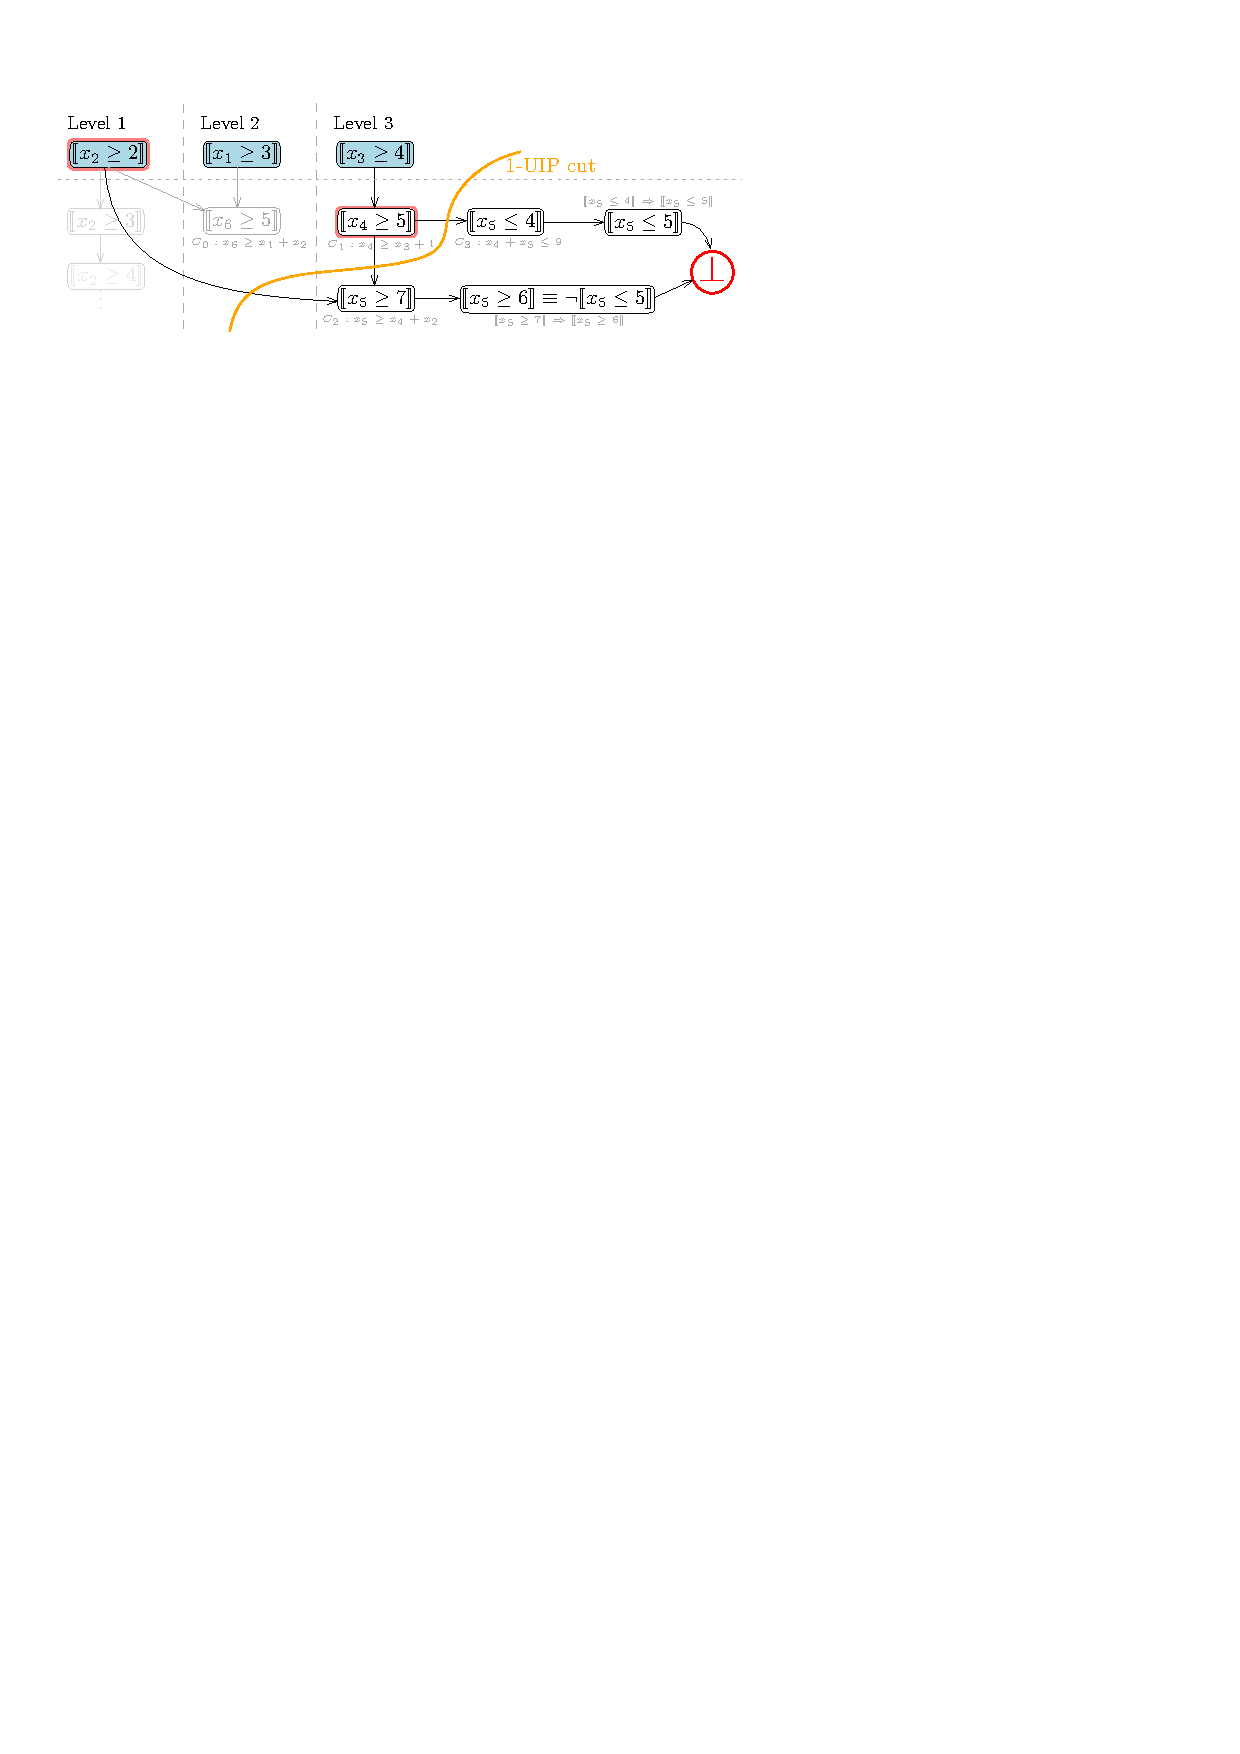
\includegraphics[width=\linewidth]{figures/conflict_analysis.pdf}
\caption{Implication graph for the trace: nodes are bound literals
$\bl{\cdot}$, blue for decisions and $\bot$ for the conflict, with the rule that
forced each propagated bound beneath it. The orange \emph{1-UIP cut} isolates the
dominator $x_4 \ge 5$ and the lower-level decision $x_2 \ge 2$ (ringed), whose
negation $\{\lnot\bl{x_4 \ge 5},\ \lnot\bl{x_2 \ge 2}\}$ is the learned nogood;
the faded branch is the off-path $x_6 \ge 5$ that analysis never visits.}
\label{fig:uipgraph}
\end{figure}

\textbf{The resolution.} Before the walk, one convention is worth stating. Each
bound on the trail holds as a \emph{true} fact, such as the $x_4 \ge 5$ the solver
set, whereas the clauses it appears in, both the failing clause and the reasons,
carry the corresponding \emph{negated} bound literal. Resolving on $x_4 \ge 5$
therefore means cancelling $\lnot\bl{x_4 \ge 5}$ in the working
clause against $\bl{x_4 \ge 5}$ in its reason. The
$\textsc{Reason}(\ell)$ the loop calls is a dispatch, not a lookup in some shared
table: when a propagator enqueues a bound it stamps that trail entry with its own
identifier, so the trail records which propagator set each $\ell$. Asking for
$\textsc{Reason}(\ell)$ calls exactly that propagator back to explain its
deduction, building the justifying clause on demand and caching it
(\srcla{sat\_base.h}{951}{Trail::Reason}, which indexes \code{propagators\_}
by the stored setter and invokes its \code{Reason}); decisions and unit facts
carry an empty reason and end the walk. This is the lazy clause generation of
\cref{sec:learning} at work: the reason exists only once conflict analysis
asks the propagator that produced $\ell$ for it. With this
convention in place, the algorithm keeps a working clause, initially the failing
clause, and repeatedly replaces the most recently assigned current-level bound by
its reason until exactly \textbf{one} current-level bound remains. It processes
bounds by decreasing trail index, which peels the conflict backward toward the
dominator. Formally, this is a short resolution loop:

\begin{algorithm}[htbp]
\caption{First-UIP conflict analysis (\code{ComputeFirstUIPConflict})}
\label{alg:uip}
\begin{algorithmic}[1]
\State $C \gets$ failing clause \Comment{the violated constraint}
\While{$C$ has more than one literal assigned at the current decision level}
  \State $\ell \gets$ the current-level literal of $C$ with the highest trail index
  \State $C \gets \big(C \setminus \{\ell\}\big) \,\cup\, \big(\textsc{Reason}(\ell) \setminus \{\lnot\ell\}\big)$ \Comment{reason = ask the propagator that set $\ell$}
\EndWhile
\State $u \gets$ the unique current-level literal remaining in $C$ \Comment{the 1-UIP}
\State \Return $C$ \Comment{learned nogood; backjump to \textnormal{\textsc{AssertionLevel}}$(C)$}
\end{algorithmic}
\end{algorithm}

Walking that loop on our trail makes the mechanics concrete:

\begin{itemize}
  \item \textbf{Start.} The working clause is the failing clause, the order-encoding
  consistency clause $\{\lnot\bl{x_5 \ge 7},\ \lnot\bl{x_5
  \le 5}\}$: the monotone link $\bl{x_5 \ge 7}
  \Rightarrow \bl{x_5 \ge 6}$, written with $\lnot\bl{x_5
  \le 5}$ in place of the bound literal $\bl{x_5 \ge 6}$ it
  equals. Both bounds were assigned at the current level, level 3, so the loop
  continues.
  \item \textbf{Resolve on $x_5 \ge 7$} (highest trail index, position 5). Its
  reason is $C_2$ acting on $x_4 \ge 5$ and $x_2 \ge 2$, giving the clause
  $\{\lnot\bl{x_4 \ge 5},\ \lnot\bl{x_2 \ge 2},\
  \bl{x_5 \ge 7}\}$, which says that $x_4 \ge 5$ and $x_2 \ge 2$
  together force $x_5 \ge 7$. Replacing $\lnot\bl{x_5 \ge 7}$ by
  the rest of that reason (writing $\odot$ for resolution) gives
  \[
    \begin{aligned}
    \{\lnot\bl{x_5 \ge 7},\ \lnot\bl{x_5 \le 5}\}
    &\odot
    \{\lnot\bl{x_4 \ge 5},\ \lnot\bl{x_2 \ge 2},\
      \bl{x_5 \ge 7}\} \\
    &= \{\lnot\bl{x_5 \le 5},\ \lnot\bl{x_4 \ge 5},\ \lnot\bl{x_2 \ge 2}\}.
    \end{aligned}
  \]
  Two current-level bounds remain, $x_5 \le 5$ and $x_4 \ge 5$, so the loop
  continues.
  \item \textbf{Resolve on $x_5 \le 5$} (position 4). This is the order-encoding
  step: $x_5 \le 5$ was forced not by a constraint but by the monotone link
  $x_5 \le 4 \Rightarrow x_5 \le 5$, whose clause is $\{\lnot\bl{x_5 \le 4},\ \bl{x_5 \le 5}\}$. Replacing $\lnot\bl{x_5
  \le 5}$ gives
  \[
    \begin{aligned}
    \{\lnot\bl{x_5 \le 5},\ \lnot\bl{x_4 \ge 5},\
      \lnot\bl{x_2 \ge 2}\}
    &\odot
    \{\lnot\bl{x_5 \le 4},\ \bl{x_5 \le 5}\} \\
    &= \{\lnot\bl{x_5 \le 4},\ \lnot\bl{x_4 \ge 5},\ \lnot\bl{x_2 \ge 2}\}.
    \end{aligned}
  \]
  The bounds $x_5 \le 4$ and $x_4 \ge 5$ are both current-level, so the loop
  continues.
  \item \textbf{Resolve on $x_5 \le 4$} (position 3). Its reason is $C_3$ acting on
  $x_4 \ge 5$, giving the clause $\{\lnot\bl{x_4 \ge 5},\
  \bl{x_5 \le 4}\}$, which says that $x_4 \ge 5$ forces
  $x_5 \le 4$. Replacing $\lnot\bl{x_5 \le 4}$ gives
  \[
    \{\lnot\bl{x_5 \le 4},\ \lnot\bl{x_4 \ge 5},\
      \lnot\bl{x_2 \ge 2}\}
    \odot
    \{\lnot\bl{x_4 \ge 5},\ \bl{x_5 \le 4}\}
    = \{\lnot\bl{x_4 \ge 5},\ \lnot\bl{x_2 \ge 2}\}.
  \]
  Only $x_4 \ge 5$ is now a current-level bound, since the other, $x_2 \ge 2$,
  belongs to level 1. Exactly \textbf{one} current-level bound remains, so the
  loop stops.
\end{itemize}

\textbf{The UIP.} The single remaining current-level bound is the
\textbf{first Unique Implication Point}, $x_4 \ge 5$. It is the one node at level
3 through which every conflict path runs, since both $x_5 \ge 7$ and $x_5 \le 5$
were forced by it. Negating it and moving it to the front gives the learned
clause
\[
  \textbf{Learned nogood: }
  \{\lnot\bl{x_4 \ge 5},\ \lnot\bl{x_2 \ge 2}\},
\]
which reads ``never have $x_4 \ge 5$ and $x_2 \ge 2$ at once,'' or equivalently
that whenever $x_2 \ge 2$ holds the bound $x_4 \le 4$ must follow. This is a fact
stated purely in bounds, sound everywhere in the tree rather than only on this
branch.

\textbf{Backjump.} The solver computes the \textbf{assertion level}: the highest
decision level among the learned clause's literals \emph{other than} the UIP
(\srcla{sat\_solver.cc}{1896}{ComputePropagationLevel}). Here that is the
level of $x_2 \ge 2$, namely level~1, so the solver retreats from level 3 straight
to level 1. Everything above level 1 is undone in the process: the level-2
decision $x_1 \ge 3$ and its propagation $x_6 \ge 5$ are popped along with the
level-3 cascade. Nothing in between is selectively kept; the undo is a plain
truncation of both trails to the end of level 1, leaving only level 1 and below.
The force of the \textbf{non-chronological backjump} is not that $x_1 \ge 3$
survives but that the solver does not stop at level 2 to retry it: that decision
had no part in the failure, so search resumes at level 1 instead.
One-level-at-a-time CP backtracking cannot make that jump.

\textbf{Assertion.} Back at level 1, $x_2 \ge 2$ is still true. So in the learned
clause $\{\lnot\bl{x_4 \ge 5},\ \lnot\bl{x_2 \ge 2}\}$ the literal $\lnot\bl{x_2 \ge 2}$ is false and
$\lnot\bl{x_4 \ge 5}$ is the only unassigned literal. The clause
is now \textbf{unit} and immediately propagates it, forcing $x_4 \le 4$
(\srcla{sat\_solver.cc}{486}{AddLearnedClauseAndEnqueueUnitPropagation}).
Search resumes already knowing a fact that cost one conflict to learn, and that
fact will fire automatically in every future branch where $x_2 \ge 2$ holds.

\textbf{Two finishing touches CP-SAT applies in practice:}

\begin{itemize}
  \item \textbf{Minimization.} Before storing the clause, CP-SAT applies
  self-subsuming resolution (\srcla{sat\_solver.cc}{2627}{MinimizeConflict}): any literal whose own reason is already implied
  by the other clause literals can be dropped, yielding a shorter, stronger
  nogood.
  \item \textbf{LBD scoring.} The clause's LBD is recorded
  (\srcla{sat\_solver.cc}{1926}{ComputeLbd}). Here the learned clause
  touches two distinct decision levels, so its LBD is 2. A low LBD marks it as a
  high-quality clause: it is more likely to be protected from clause-database
  cleanup, and it later feeds the restart heuristic (\cref{sec:restarts}).
\end{itemize}

That one trace exercises every part of the engine: propagators deduce with
reasons, the conflict resolves those reasons to a unique dominator, the
dominator becomes a permanent learned clause, and a non-chronological backjump
turns the lesson into immediate forward progress.

% Source (VERIFIED): "Search stats" table column "Conflicts" = FormatCounter(r.num_conflicts())
%   in ortools/sat/stat_tables.cc:91. The response field "conflicts:"
%   (cp_model_solver.cc:712) is NOT a portfolio sum -- it is one worker's
%   num_failures(), copied by the statistics postprocessor (see the portfolio box in
%   the parallelization section); a real 24-worker log showed conflicts:0 in the
%   summary while the 'core' row recorded ~920k.
% Empirical (real CP-SAT logs): Conflicts <= Branches in EVERY worker observed
%   (a conflict is resolved by a backjump that undoes >=1 decision). The diagnostic
%   is the ratio: Conflicts ~ Branches => learning from almost every decision;
%   Conflicts << Branches (or 0) => mostly feasible descent.
\begin{platypuslog}[htb]
Each conflict resolution increments the \code{Conflicts} column of the per-worker
\textsf{Search stats} table: one learned nogood per conflict. In ordinary search,
a conflict is resolved by a backjump that undoes at least one decision, so
\code{Conflicts} stays at or below \code{Branches} in each worker. The useful
diagnostic is how close the two counts are. A \code{Conflicts} count that is a
large fraction of \code{Branches} indicates a worker learning from nearly every
decision; \code{Conflicts} tiny compared with \code{Branches}, or zero, indicates
a worker mostly descending feasibly without hitting dead ends.
\end{platypuslog}

\section{Lazy integer encoding}\label{part:encoding}

The conflict analysis of \cref{sec:learning} resolved over Boolean bound
literals such as $\bl{x_5 \ge 6}$ and learned clauses written in them, taking for
granted that those Booleans exist. This section describes where they come from:
the part of CP-SAT that reconciles an integer variable with a huge domain with a
CDCL engine that ultimately reasons in Boolean literals.

The lazy-reason machinery of the preceding sections only works because the
Boolean layer it feeds is itself built lazily: an integer variable's encoding
into Booleans is created on demand, the same way its reasons are. That is why it
follows learning directly rather than waiting among the later accelerators.

The encoding below puts one Boolean on each bound $\bl{x \ge v}$, which looks like a \emph{unary} encoding: a variable over a million
values would seem to need a million Booleans, the very blow-up a binary encoding
exists to avoid. The resolution is the word \emph{lazy}. CP-SAT never lays down
that unary chain in full; it mints a bound literal only at the moment some
mechanism actually refers to it, so a wide integer typically contributes a
handful of Booleans rather than its whole range. The encoding is unary in
\emph{form} but sparse in \emph{practice}, and the rest of this section is about
how that sparsity is achieved and what it costs elsewhere.

It also helps to be precise about what kind of mechanism this is. Lazy clause
generation (\cref{sec:learning}) is a \textbf{correctness} mechanism:
reasons are what make learned clauses sound deductions. Lazy \emph{encoding}, by
contrast, is an \textbf{efficiency} mechanism: CP-SAT would stay correct if it
encoded every bound up front. Whether that would even hurt depends on the
domains involved. Many models are dominated by Boolean variables, and a variable
with a small domain costs only a few bound literals; there, eager encoding
would do no real harm. The cost concentrates on the variables whose domains are
genuinely wide. The objective is the usual one (a weighted sum can range over
millions), and CP-SAT mints further wide-domain integers of its own when it
breaks a long linear constraint into a tree of partial sums. Encode every
bound of those up front and the model turns slow and memory-hungry.

\subsection{Minting Booleans on demand}\label{sec:encoding}
% Sources (VERIFIED): ortools/sat/integer.h, ortools/sat/integer.cc
%   IntegerEncoder; GetOrCreateAssociatedLiteral() (order/"list" encoding,
%   adds implications to neighbor literals; comment cites Feydy & Stuckey,
%   "Lazy Clause Generation Reengineered", CP 2009);
%   GetOrCreateLiteralAssociatedToEquality(); FullyEncodeVariable() (eager path);
%   Canonicalize() (folds domains with holes); NegationOf() shares the encoding;
%   num_created_variables_ counts created Booleans.
%   ortools/sat/integer_search.cc -- GetDecisionLiteral() calls
%     GetOrCreateAssociatedLiteral when branching (one of the two creation sites).
%   ortools/sat/integer_resolution.cc -- the other creation site (1-UIP).
%   ortools/sat/cp_model_loader.cc -- ExtractEncoding() creates value literals
%     (x == v) up front during loading/presolve (value encoding is STATIC).

\textbf{Why eager encoding is hopeless.} The naive bridge would give every
bound its own Boolean up front. A variable $x \in [0, 10^6]$ would spawn a
million literals
\[
  \bl{x \ge 1},\quad
  \bl{x \ge 2},\quad
  \ldots
\]
before search even starts. This is a non-starter in both memory and propagation
cost, and the overwhelming majority of those literals would never be touched.
CP-SAT therefore does not pre-encode all bounds. The integer trail reasons
about bounds \emph{directly}, as native integer facts
(\cref{sec:bounds}), and Booleans are created only where the integer and
Boolean worlds actually need to meet.

\textbf{The order encoding.} When that bridge is built, it uses the
\emph{order encoding}, also called the ``list encoding.'' CP-SAT follows Feydy
and Stuckey's \emph{``Lazy Clause Generation Reengineered''} (CP
2009)~\cite{feydy2009lcg}.
% The code comment at integer.h:106 attributes the order encoding to this paper.
For a variable $x$, the bound
literals have the form $\bl{x \ge v}$, and they are linked by
the obvious monotone implications:
\[
  \bl{x \ge 6} \;\Rightarrow\; \bl{x \ge 5}
  \;\Rightarrow\; \bl{x \ge 4} \;\Rightarrow\; \cdots .
\]
A single such Boolean also represents the corresponding upper-bound fact,
because
\[
  \bl{x \le v}
  \equiv
  \lnot\bl{x \ge v{+}1} .
\]
In the implementation, the upper-bound side is handled by sharing the encoding
with \code{NegationOf}$(x)$, so $x$ and its negation do not duplicate Booleans.

\textbf{On-demand creation.} The workhorse is
\srcla{integer.h}{193}{GetOrCreateAssociatedLiteral}$(x \ge v)$. It
returns the Boolean $\bl{x \ge v}$. If that literal does
not yet exist, it mints a fresh Boolean variable and wires in the implications to
the already encoded neighboring bounds, the next bound below and the
next bound above. This preserves the monotone chain.

This is the moment alluded to in the conflict trace of \cref{sec:trace}.
When 1-UIP resolution needs $\bl{x \ge v}$ as a clause literal, this call
materializes it. The implication links keep it consistent
with its neighbors, and from then on the SAT engine treats it like any other
Boolean literal. In the basic search loop, two moments dominate bound-literal
creation: \emph{branching} on an integer bound mints the Boolean for that
bound (\srcla{integer\_search.cc}{1426}{GetDecisionLiteral}), and
\emph{integer conflict resolution} mints the Boolean it needs for the 1-UIP
(\cref{sec:trace}). Other mechanisms call the same
\code{GetOrCreateAssociatedLiteral} on demand as well, including core-guided
optimization when forming assumption literals, the feasibility pump, and some
global propagators. Ordinary bound propagation, however, stays in integer-bound
space and creates no Booleans. That is what keeps the Boolean skeleton small.

\textbf{Equality literals.} Some constraints, for example a table constraint,
\srcla{all\_different.h}{52}{AllDifferent}, or anything that reasons about exact
values, want $\bl{x = v}$, not just bounds.
\srcla{integer.h}{194}{GetOrCreateLiteralAssociatedToEquality}$(x, v)$
provides it, based on the identity
\[
  \bl{x = v} \;\Longleftrightarrow\;
  \bl{x \ge v} \;\wedge\; \bl{x \le v} .
\]
A constraint may even ask for the whole domain at once via
\srcla{integer.h}{144}{FullyEncodeVariable}. This is the deliberate
\emph{eager} path, used precisely when a propagator is going to need every value
anyway, so laziness would only add overhead. Full encoding is the exception
requested by a constraint; lazy bound encoding is the default for everything
else.

There is an important asymmetry between the two encodings. The bound literals
$\bl{x \ge v}$ of the order encoding are predominantly \emph{dynamic}: they
are minted during branching and conflict resolution as just described. Value
literals $\bl{x = v}$ are predominantly \emph{static}: the
equalities a model needs are detected and created up front during
presolve/loading (\srcla{cp\_model\_loader.cc}{352}{ExtractEncoding}), rather
than on demand. That said,
\code{GetOrCreateLiteralAssociatedToEquality} can still mint one lazily if a
constraint later asks for a value literal that loading did not foresee. The
developers' rule of thumb behind this split is blunt: if a model genuinely needs
per-value Booleans for a variable, that variable probably should not have been a
wide integer in the first place.

\textbf{Domains with holes.} Real domains are not always intervals. If
$x \in [1,2] \cup [5,6]$, then ``$x \le 3$'' and ``$x \le 4$'' mean the same
thing as ``$x \le 2$,'' and ``$x \ge 3$'' means ``$x \ge 5$.'' The encoder's
\srcla{integer.h}{177}{Canonicalize} step folds each requested bound onto
the canonical bound for that domain before looking it up. Equivalent bounds
therefore share one Boolean instead of spawning redundant ones.

\textbf{The payoff.} The Boolean skeleton that the CDCL engine actually sees
stays small: it contains only the bounds and equalities that branching,
conflict learning, or a constraint-specific encoding genuinely reached. A
variable over a million values typically contributes a handful of literals, not
a million, and the encoder tracks exactly how many Booleans it had to create
(\code{num\_created\_variables\_}). Both layers are lazy: the reasons
(\cref{sec:learning}) and the Boolean variables they are written in.
Strong integer propagation does
the bulk of the reasoning natively over bounds, and the Boolean encoding
materializes only at the thin interface where the learning machinery needs to
grip.

% Source (VERIFIED): "Search stats" column "Bools" = FormatCounter(r.num_booleans())
%   in ortools/sat/stat_tables.cc:90. The response field "booleans:"
%   (cp_model_solver.cc:711) is one worker's SatSolver::NumVariables(), not a
%   portfolio figure -- different workers mint different amounts (see the portfolio
%   box in the parallelization section).
\begin{platypuslog}[htb]
The size of the lazily minted Boolean skeleton is reported per worker as the
\code{Bools} column of the \textsf{Search stats} table; each worker mints its own,
so the counts differ across rows. For a model with wide integer domains it usually
stays orders of magnitude below the number of representable values: the measurable
payoff of minting bound literals on demand rather than up front.
\end{platypuslog}

\subsection{A fixed skeleton need not be a solution}\label{sec:completion}
% Sources (VERIFIED):
%   ortools/sat/integer_search.cc:422 SatSolverHeuristic -- all_assigned =
%     trail->Index() == sat_solver->NumVariables(); returns no decision when true.
%   The completion heuristic that closes this gap (AtMinValue, bisection, LP
%   value; completion-last policy) is assembled in sec:search.

The sparse skeleton has a consequence the foundational search of
\cref{sec:complete} sidestepped. Because the skeleton holds only a handful
of bounds, all of them can be assigned while an integer still spans a range:
$\bl{x \ge 3}$ true and $\bl{x \ge 8}$ false
leave $x \in [3,7]$ with every \emph{existing} literal decided. The gap is then a
\emph{missing} literal, not an unassigned one. Even a complete Boolean assignment
can leave $x$ genuinely ranged, because no bound between $3$ and $7$ was ever
minted. Under a full encoding this could not arise, since deciding every
bound pins the value; the sparse skeleton is exactly what pulls the two
tests apart.

Closing this gap is the job of \emph{integer completion}, the second half of the
search machinery in \cref{sec:search}: once the Boolean skeleton is
settled but some integer is still ranged, the solver mints a fresh bound for
that integer and branches on it, repeating until every variable is pinned to a
single value.

\section{Putting it together}\label{part:together}

This section assembles the moving parts into a single control loop: bounds and
their literals (\cref{part:foundations}), propagators that tighten them, branching
that commits values, and conflict analysis that learns from failure
(\cref{part:learning}). It then opens the loop's two busiest lines: what
``propagate to a fixed point'' actually runs, and in what order the SAT and CP
engines take turns (\cref{sec:propstep}); and how the next decision is
chosen once propagation stalls, where a deliberate design choice has CP-SAT drive
the search itself and lets a configurable decision strategy, by default led by SAT
branching, choose where to descend (\cref{sec:search}).

\subsection{The search loop, assembled}\label{sec:loop}
% Sources (VERIFIED):
%   ortools/sat/integer_search.cc -- main integer search loop: repeatedly
%     propagate, take a decision, on conflict analyze+backjump; return FEASIBLE
%     when the heuristic yields no decision (all variables fixed).
%   ortools/sat/sat_solver.cc -- SatSolver::Solve / Propagate / conflict handling.
%   ortools/sat/optimization.cc -- the objective-tightening wrapper around it.

Putting the pieces together, the engine is a single feasibility loop
(\srcla{integer\_search.cc}{1526}{SolveIntegerProblem}, entered through the
level-$0$ reset-and-assert wrapper
\srcla{integer\_search.cc}{1649}{ResetAndSolveIntegerProblem}) wrapped by a
thin optimizer that calls it repeatedly. The loop, \textsc{Solve}
(\cref{alg:loop}), is the heart:
every concept introduced so far appears in it exactly once, and each line points to
a section that expands it. It takes a set of \emph{assumptions} (literals forced
true for the duration of one call) and returns either a feasible solution or a
proof that none exists under them. The wrapper,
\textsc{MinimizeByBisection} (\cref{alg:bisection}), turns that feasibility engine into an optimizer: it
calls \textsc{Solve} under a trial bound on the objective and narrows that bound by
bisection until the optimum is pinned.

\begin{algorithm}[htbp]
\caption{The CP-SAT feasibility core, \textsc{Solve}}
\label{alg:loop}
\begin{algorithmic}[1]
\Procedure{Solve}{$A$} \Comment{$A$: assumption literals, forced true for this call}
  \LineComment{Prepare the model for a new run, with the assumptions enforced at the root level}
  \State reset to decision level $0$; assert every $\ell \in A$
  \Loop
    \LineComment{Run all propagators (cheapest first) until we reach a fixed point (\cref{sec:propstep})}
    \State \Call{PropagateToFixedPoint}{} \Comment{first SAT, then CP propagations}
    \If{conflict detected}
      \LineComment{Learn from the conflict and resolve it (\cref{sec:trace})}
      \If{current decision level $= 0$}
        \State \Return \textsc{Infeasible} \Comment{with the failing core $\subseteq A$, when $A \neq \emptyset$}
      \EndIf
      \State $c \gets \Call{AnalyzeConflict}{}$ \Comment{1-UIP nogood}
      \State \Call{Backjump}{\textsc{AssertionLevel}$(c)$}; \ \Call{Learn}{$c$}
    \Else
      \LineComment{Ask the decision strategies for a branching literal, or confirm none is left (\cref{sec:search})}
      \State $\ell \gets \Call{NextDecision}{}$ \Comment{default: (1)~VSIDS, (2)~integer completion}
      \If{$\ell = \textsc{none}$} \Comment{everything well-defined: a full solution}
        \State \Return \textsc{Feasible}(current assignment)
      \EndIf
      \State \Call{Assert}{$\ell$} \Comment{descend one decision level}
    \EndIf
  \EndLoop
\EndProcedure
\end{algorithmic}
\end{algorithm}

% Source (VERIFIED): ortools/sat/optimization.cc:259
%   RestrictObjectiveDomainWithBinarySearch -- assumption =
%   GetOrCreateAssociatedLiteral(LowerOrEqual(objective_var, target)),
%   ResetAndSolveIntegerProblem({assumption}); on FEASIBLE restrict ub to the
%   solution's objective, on ASSUMPTIONS_UNSAT Enqueue(GreaterOrEqual(obj,target+1)).
\begin{algorithm}[htbp]
\caption{Optimization by bisection: \textsc{MinimizeByBisection} drives \textsc{Solve}}
\label{alg:bisection}
\begin{algorithmic}[1]
\Procedure{MinimizeByBisection}{$\code{obj}$}
  \State $\text{lo} \gets \text{lb}(\code{obj})$; \ $\text{hi} \gets \text{ub}(\code{obj})$; \ \textit{incumbent} $\gets \textsc{none}$
  \While{$\text{lo} < \text{hi}$}
    \State $m \gets \lfloor (\text{lo} + \text{hi})/2 \rfloor$
    \State $r \gets \Call{Solve}{\{\bl{\code{obj} \le m}\}}$ \Comment{assume the trial bound for one call}
    \If{$r = \textsc{Infeasible}$}
      \State $\text{lo} \gets m + 1$ \Comment{the returned core proves $\code{obj} > m$}
    \Else
      \State \textit{incumbent} $\gets r$; \ $\text{hi} \gets \code{obj}(\textit{incumbent})$ \Comment{a solution of cost $\le m$}
    \EndIf
  \EndWhile
  \State \Return \textit{incumbent} as \textsc{Optimal}
\EndProcedure
\end{algorithmic}
\end{algorithm}

The two procedures factor the engine cleanly. \textsc{Solve}'s contract is
feasibility: it returns a feasible assignment or a proof none exists, and it never
manages the objective bound --- that bookkeeping is entirely the wrapper's. The
loop itself carries no optimization logic; the only cost-awareness inside it lives
in the decision strategies, which can be set up, explicitly or implicitly, to
branch toward cheaper solutions (\cref{sec:search}). \textsc{MinimizeByBisection}
(\srcla{optimization.cc}{259}{RestrictObjectiveDomainWithBinarySearch}) keeps a
lower and an upper bound on the
optimal cost and, each round, asks \textsc{Solve} whether a solution of cost at most
the midpoint $m$ exists --- forcing the order-encoding literal
$\bl{\, \code{obj} \le m \,}$ (minted on demand by
\srcla{integer.h}{193}{GetOrCreateAssociatedLiteral}) as an \emph{assumption}, a fact held
only for that one call. This works because the objective is just one more bounded
integer variable (\cref{sec:opt}) and a bound \emph{is} a literal
(\cref{part:foundations}). The two answers move opposite ends of the gap: a solution
pulls the upper bound down to its cost, while an \textsc{Infeasible} hands back a
\emph{core} --- the subset of the assumptions that cannot hold together --- proving
$\code{obj} > m$ and lifting the lower bound. When the two bounds meet, the incumbent
is optimal, and that final infeasibility proof \emph{is} the proof of optimality.
This is the first place \textsc{Solve}'s assumption input and core output earn their
keep; \cref{sec:opt} puts the same $A$ parameter to work in the other
strategies that drive this loop.

This single loop hides a deeper design decision: how the CDCL clause-learning
machinery is coupled to finite-domain propagation. There are broadly two ways to
wire the two together. One option is to keep a complete CDCL \textbf{SAT solver in
charge} and let it own the whole search stack: the trail, the decisions, unit
propagation, conflict analysis, and backjumping. The finite-domain side then talks
to it only through the clause interface, injecting fresh clauses (and the Boolean
variables they need) whenever it notices the solver has missed something a
constraint implies. The SAT engine runs the show; the constraint reasoning feeds
it from outside.

CP-SAT takes the other option: it \textbf{drives the search itself}. It runs its
own propagation, conflict analysis, and search as one integrated core, and the
CDCL clause-learning machinery is a mechanism inside that core rather than an
external engine being fed from the side. This choice runs through every line of
the loop. Boolean literals and integer bounds share one decision-level timeline across two
coupled trails (\cref{sec:trail}), so the \textsc{PropagateToFixedPoint} step runs the CP
propagators directly and a finite-domain propagator pushes an integer-bound fact
onto the integer trail itself (\cref{sec:propstep}); conflict analysis then resolves
over those integer literals natively, and the Boolean clauses and variables are
minted lazily, only at the thin interface where the two worlds meet. This is what
lets the costly apparatus of \cref{part:learning} pay off: a decision and the
reason later learned from it are written in the very same literals, so every
failure feeds straight back into the search that produced it, with no re-encoding
round trip.

The interesting work inside \textsc{Solve}'s conflict case is split between
\textbf{learning} and \textbf{backjumping}. Branching is not a single rule but a walk down an ordered
\textbf{decision strategy} $\mathcal{S}$, a list of heuristics: \textsc{NextDecision}
tries each in turn and returns the first literal one produces, which the loop then
asserts. By default $\mathcal{S}$
holds two such heuristics (\cref{sec:search}): the SAT decision heuristic
(\textbf{VSIDS}), which keeps branching on existing bound literals until every one
has a value, and \textbf{integer completion}, a generic fallback that takes the
first variable still spanning a range and fixes it toward its minimum. Running only
after VSIDS has settled every Boolean, completion in practice sees just the integers
the skeleton has left loose, minting one bound at a time until each domain
collapses to a single value. The loop reports a solution only when \emph{every} heuristic in
$\mathcal{S}$ comes up empty, which is why the leaf test is stricter than ``all
Booleans assigned'': it holds only once every domain has also shrunk to a
singleton.

Which heuristics $\mathcal{S}$ contains, and in what order, is part of the
configuration rather than a fixed feature of the loop. \cref{sec:search}
takes the strategy apart: what each of the two default heuristics does, and how
the parallel portfolio reorders and extends them across workers.

% Source (VERIFIED): the "Search stats" table is built in ortools/sat/stat_tables.cc:84-92
%   (header "...Branches..."; FormatCounter(r.num_branches())). The response field
%   "branches:" (cp_model_solver.cc:713) is NOT a portfolio sum: it is one worker's
%   num_branches(), copied by the statistics postprocessor (see sec:portfolio).
% Empirical (checked against real CP-SAT logs): per-worker Branches has NO fixed
%   relation to the variable count -- orders of magnitude ABOVE it (hard small models,
%   restart/backjump re-descents) or far BELOW it (large models solved at the root).
%   In xl_20x6_120parties.log the response showed branches:1072 (below 2730 vars)
%   because the solution-holding worker barely searched.
\begin{platypuslog}[htb]
Each pass through the \textsc{Assert} line is counted as a \code{Branch} in the
per-worker \textsf{Search stats} table printed at the end of a run. The count has
no fixed relation to the number of variables: it tallies decisions over the
\emph{whole} search, so restarts and backjumping can drive a searching worker to
many times the variable count, while a worker that rides presolve and root
propagation can finish with far fewer. Within one worker's row it sits well below
the two propagation columns beside it (\cref{sec:propstep}): every decision sets
off a full cascade, so \code{BoolPropag} and \code{IntegerPropag} both run far
ahead of \code{Branches} wherever real search happens. Read these per worker; the
response summary's \code{branches:} field reports only the worker that returned
the solution (\cref{sec:portfolio}), which can be far smaller.
\end{platypuslog}

\textsc{Solve} and its optimizer, together with strong propagators, are the search
core. Bisection is one clean way to drive the feasibility loop;
\cref{sec:opt} surveys the others, including the even simpler linear scan and
the core-guided strategies the portfolio runs.

\subsection{Inside ``propagate to a fixed point''}\label{sec:propstep}
% Sources (VERIFIED):
%   ortools/sat/sat_solver.cc -- SatSolver::Propagate(): loops over an ordered
%     propagators_ list; the inner loop BREAKS as soon as the trail grows, so it
%     restarts from the cheapest propagator. Registration order: binary_implication_graph_,
%     clauses_propagator_, enforcement_propagator_, pb_constraints_, external,
%     then GenericLiteralWatcher (last_propagator_). The in-source comment states
%     the intent ("loop over and test again the highest priority constraint types").
%   ortools/sat/clause.cc -- BinaryImplicationGraph::Propagate() and
%     ClauseManager::Propagate() ARE the unit-propagation engines (the "first row").
%   ortools/sat/integer.cc -- GenericLiteralWatcher::Propagate(): priority buckets
%     queue_by_priority_ (default priority 1; 0 = cheap), drains low priority first,
%     resets to priority 0 when an integer bound is enqueued, RETURNS to the SAT
%     loop when a Boolean literal is enqueued.
%   ortools/sat/integer.h -- WatchLiteral/WatchLowerBound/WatchUpperBound +
%     PropagatorInterface::IncrementalPropagate(watch_indices): change-driven waking.

The loop of \cref{sec:loop} hides its most important line:
``propagate to a fixed point.'' What actually happens there, and where does the
SAT engine sit relative to the CP propagators?

\begin{platypuswarning}[htb][Not generate-and-check]
CP-SAT does \emph{not} let the SAT solver guess a complete Boolean assignment
and then hand it to the CP propagators for checking, as in generate-and-check
lazy SMT or CEGAR. Propagation is \textbf{online}: it runs after \emph{every}
decision, before the next one, and the propagators always operate on the current
\emph{partial} state, namely the bounds as they stand, never on a finished
assignment.
\end{platypuswarning}

\textbf{A layered, cheapest-first cascade.} Propagators are kept in a fixed
order, with the cheapest and most prolific first, and the engine runs them as a
chain:

\begin{enumerate}[leftmargin=1.6em,topsep=0.3em,itemsep=0.25em]
  \item the \textbf{binary-implication graph}: implications from two-literal
  clauses, the cheapest form of unit propagation;
  \item the \textbf{clause manager}: unit propagation on general clauses via the
  two-watched-literals scheme;
  \item enforcement and \textbf{pseudo-Boolean} constraints;
  \item the \textbf{\srcla{integer.h}{1324}{GenericLiteralWatcher}}, which fans
  out to all integer and CP propagators: linear,
  \srcla{all\_different.h}{52}{AllDifferent},
  \srcla{disjunctive.h}{49}{NoOverlap},
  \srcla{cumulative.h}{48}{Cumulative}, and so on.
\end{enumerate}

The first two layers \emph{are} classical SAT unit propagation. This is the
``first-row propagator'' picture: cheap, always-run Boolean reasoning fires
before any expensive global constraint is even consulted.

\textbf{Restart-on-progress is the key scheduling rule.} The instant any
propagator deduces something new, by enqueuing a literal or tightening a bound,
the chain breaks and starts again \emph{from the top}. Thus, when an expensive
global constraint such as \srcla{cumulative.h}{48}{Cumulative} tightens a bound,
control immediately returns to binary-implication and clause unit propagation.
Those cheap layers then run to their own fixed point again before any expensive
propagator is reconsidered. Cheap reasoning is always exhausted before the
engine spends time on expensive reasoning.

The same discipline repeats one level down inside
\srcla{integer.h}{1324}{GenericLiteralWatcher}. CP propagators are themselves
bucketed by priority: priority 0 for cheap propagators such as linear and
scheduling helpers, and higher priorities for more expensive propagators such as
\srcla{all\_different.h}{52}{AllDifferent} or
\srcla{cumulative.h}{48}{Cumulative}. The watcher drains priority 0 before
priority 1, but resets to priority 0 as soon as a cheap propagator tightens a
bound. If a propagator pushes a \emph{Boolean} literal, control returns to the
SAT layer immediately, so unit propagation re-runs before anything costlier.

\textbf{Change-driven waking.} None of this rescans every constraint in every
round. At registration, a propagator declares exactly which literals and
variable bounds it cares about (\srcla{integer.h}{1369}{WatchLiteral}, \srcla{integer.h}{1370}{WatchLowerBound},
\srcla{integer.h}{1371}{WatchUpperBound}). It is then woken only when one of \emph{those} facts
changes, and it receives the changed watch indices through
\srcla{integer.h}{1299}{IncrementalPropagate} rather than recomputing from scratch. The fixed-point
loop is therefore sparse: only the constraints touched by the last deduction are
re-run, and they are usually told precisely what moved.

Putting this together, a single decision triggers a cascade that first exhausts
the cheapest propagation, escalates to expensive global constraints only when
the cheap layers stall, returns to cheap propagation the moment anything new is
deduced, and wakes only constraints whose watched facts changed. Only when the
\emph{entire} cascade stalls does control return to branching; if some
propagator instead empties a domain, control goes to the conflict analysis of
\cref{sec:learning}.

% Source (VERIFIED): "Search stats" columns "BoolPropag"/"IntegerPropag" =
%   FormatCounter(r.num_binary_propagations())/FormatCounter(r.num_integer_propagations())
%   in ortools/sat/stat_tables.cc:96-97. The two counters come from two structures:
%   num_binary_propagations() := SatSolver::num_propagations() (Boolean trail, binary
%   + clause unit propagation), num_integer_propagations() := IntegerTrail::num_enqueues()
%   (integer trail). Naming trap: the response field is PRINTED as "propagations:" but
%   is num_binary_propagations() (cp_model_solver.cc:715-718 comment says so), the
%   Boolean count only; the response prints just ONE worker's figures (see sec:portfolio).
% Empirical (real CP-SAT logs): do NOT claim IntegerPropag > BoolPropag -- the
%   order between them flips by model (clause-heavy encodings make BoolPropag the
%   larger, e.g. 65.7M vs 36.9M). What IS robust: both > Branches in every
%   searching worker. So anchor the message on the propagation-vs-Branches gap.
\begin{platypuslog}[htb]
The two trails are tallied by two separate columns of the \textsf{Search stats}
table. \code{BoolPropag} counts propagations on the Boolean trail (the
binary-implication and clause layers), read from the SAT solver's own counter;
\code{IntegerPropag} counts bound tightenings pushed onto the integer trail, read
from that trail's enqueue count. In a worker that genuinely searches they are
usually the two largest columns by a wide margin, the quantitative face of
``propagation does most of the work, branching only a little.'' Which of the two
leads is model-dependent: clause-heavy encodings can put \code{BoolPropag} ahead,
so the message lies in their size relative to \code{Branches}, not in the split
between them. The response summary echoes the pair as \code{integer\_propagations:}
and --- a naming trap --- \code{propagations:} for the Boolean count, but, like the
other summary counters, only for the single worker that returned the solution
(\cref{sec:portfolio}).
\end{platypuslog}

\subsection{Inside ``search'': choosing the next decision}\label{sec:search}
% Sources (VERIFIED):
%   ortools/sat/sat_decision.h:58 -- VSIDS-style decaying activity, phase saving.
%   ortools/sat/integer_search.cc:422 SatSolverHeuristic -- all_assigned test
%     (returns no decision when every Boolean is assigned);
%   integer_search.cc:61 AtMinValue (min-first completion);
%   integer_search.cc:80 GreaterOrEqualToMiddleValue (bisection);
%   integer_search.cc:119 SplitAroundLpValue (LP value);
%   integer_search.cc:1224 SequentialSearch({SatSolverHeuristic, fixed_search})
%     -- completion (fixed_search) is the last heuristic in the default policy.

The companion to ``propagate to a fixed point'' is the other line the loop hides:
how the next decision is actually chosen. The integrated design of
\cref{sec:loop} --- one decision-level timeline across its two trails, with clause learning a mechanism
inside the core --- settles how decisions are represented and learned from, but
not \emph{which} heuristic picks the next one. That is the configurable decision
strategy $\mathcal{S}$ of \cref{sec:loop}: the default leads with SAT
branching and falls back to finite-domain branching, but other workers reorder
these or lead with an LP or a fixed integer order instead. The two heuristics
below are the entries of that default $\mathcal{S}$, and the building blocks the
other strategies recombine.

\textbf{The SAT decision heuristic.} This entry branches on a bound literal that
already exists. CP-SAT's SAT core chooses it by \textbf{VSIDS}
(\srcl{sat\_decision.h}{58}): it keeps a decaying activity score per variable,
bumps the variables that appear in each conflict, and branches on whichever has
been most involved in recent failures, with a saved polarity (\emph{phase
saving}) picking true or false. Because an integer bound is a reified literal
(\cref{sec:bounds}), this one heuristic ranges over Boolean and integer
variables alike: the literals it scores are exactly the bound literals conflict
analysis has been resolving over. This is the sense in which this entry branches
from the SAT side.

\textbf{Integer completion.} VSIDS can branch only on literals that already
exist, and the sparse skeleton (\cref{sec:completion}) lets those run out
while an integer is still ranged: every existing bound for $x$ is assigned,
yet $x \in [3,7]$ because no bound between $3$ and $7$ was ever minted. When
the SAT heuristic reports nothing left to decide, every Boolean is assigned
(\srcla{integer\_search.cc}{422}{SatSolverHeuristic}), and only then does an
\emph{integer-completion} heuristic step in: it picks a still-ranged variable,
mints a fresh bound for it, and branches on that. The default composition puts
completion last for exactly this reason (\srcl{integer\_search.cc}{1224}):
exhaust the existing Booleans first, and fall back to minting a new one only when
the skeleton is settled but some integer is still loose.

Which bound to mint is a value-selection choice. The default branches the
variable toward its current minimum, asserting $\bl{x \le \text{lb}(x)}$ (\srcla{integer\_search.cc}{61}{AtMinValue}): the first guess tries
the smallest surviving value, and the other branch pushes the lower bound up.
Other configurations bisect instead, minting a middle bound
$\bl{x \ge \text{lb} + \lceil(\text{ub}-\text{lb})/2\rceil}$
(\srcla{integer\_search.cc}{80}{GreaterOrEqualToMiddleValue}) to halve the range
per decision, or split around the current LP value. Each is just a rule for which
not-yet-minted bound becomes the next decision.

This is why search terminates on $\text{lb} = \text{ub}$ rather than when the
Booleans are exhausted: completion keeps minting bounds for an unfixed
variable instead of declaring victory once the SAT skeleton is satisfied. The
propagation fixed point of \cref{sec:propstep} becomes a \emph{solution}
only when every integer has been pinned to a single value, one missing literal at
a time.

\textbf{How workers vary the strategy.} These two heuristics are only the default
$\mathcal{S}$. Nothing in the loop of \cref{sec:loop} fixes \emph{which}
strategy it runs, and the parallel portfolio (\cref{sec:portfolio})
exploits this, running workers whose $\mathcal{S}$ differs in both contents and
order, selected through the \code{search\_branching} parameter:

\begin{itemize}[leftmargin=1.6em,topsep=0.3em,itemsep=0.25em]
  \item \code{auto} (\srcla{integer\_search.cc}{1224}{AUTOMATIC\_SEARCH}, the default):
  $\langle\text{VSIDS},\ \text{integer completion}\rangle$;
  \item \code{fixed} (\srcla{integer\_search.cc}{1239}{FIXED\_SEARCH}):
  $\langle\text{fixed integer order},\ \text{VSIDS}\rangle$, the integer-style
  decisions first, with VSIDS only settling any leftover Booleans;
  \item \code{reduced\_costs} (\srcla{integer\_search.cc}{1288}{LP\_SEARCH}):
  $\langle\text{LP reduced-cost},\ \text{VSIDS},\ \text{integer completion}\rangle$;
  \item \code{pseudo\_costs} (\srcla{integer\_search.cc}{1310}{PSEUDO\_COST\_SEARCH}):
  $\langle\text{pseudo-cost},\ \text{VSIDS},\ \text{integer completion}\rangle$;
  \item \code{portfolio} and \code{quick\_restart}
  (\srcla{integer\_search.cc}{1282}{PORTFOLIO\_SEARCH}, \srcla{integer\_search.cc}{1319}{PORTFOLIO\_WITH\_QUICK\_RESTART\_SEARCH}):
  a randomized rotation over such lists, reshuffled on restart.
\end{itemize}

Only the contents and order of $\mathcal{S}$ change between workers; the loop
around it does not.

% Sources (VERIFIED against sat_parameters.proto / cp_model.proto):
%   search_branching (SearchBranching enum) field 82, default AUTOMATIC_SEARCH:
%     sat_parameters.proto:1194 (field), enum 1151-1193. FIXED_SEARCH=1 (proto:1161).
%   The user-supplied fixed order is the repeated search_strategy field of the
%     CpModelProto: cp_model.proto:654 (repeated DecisionStrategyProto), message
%     DecisionStrategyProto cp_model.proto:520, VariableSelectionStrategy enum
%     :539 (CHOOSE_FIRST=0 :540, CHOOSE_LOWEST_MIN=1 :541, ...),
%     DomainReductionStrategy enum :552 (SELECT_MIN_VALUE=0 :553,
%     SELECT_MAX_VALUE=1 :554, ...). Python API: model.add_decision_strategy().
%   Caveat re portfolio: a single global search_branching binds only the workers
%     that honour it; see the subsolver-restriction box in \cref{sec:portfolio}.
\begin{platypusparam}[htb]
You can also supply your own search strategy $\mathcal{S}$ instead of leaving it to the
portfolio. The \srcla{sat\_parameters.proto}{1194}{search\_branching} parameter (default \code{AUTOMATIC\_SEARCH}) selects the policy,
and \code{FIXED\_SEARCH} makes the solver follow an order \emph{you} specify,
walked by \srcla{cp\_model\_search.cc}{210}{ConstructUserSearchStrategy}.
That order is a per-model object: each
\srcla{cp\_model.proto}{520}{DecisionStrategyProto} (the repeated
\srcla{cp\_model.proto}{654}{search\_strategy} field, exposed as
\code{add\_decision\_strategy} in the Python API) pairs a
\textbf{variable-selection} rule (\code{CHOOSE\_FIRST},
\code{CHOOSE\_LOWEST\_MIN}, \dots) with a \textbf{value} rule
(\code{SELECT\_MIN\_VALUE}, \code{SELECT\_MAX\_VALUE}, \dots), letting you
hand-encode a custom variable and value order rather than leaving the choice to
the automatic activity heuristic.
\end{platypusparam}

\subsection{A small worked example}

The following tiny model illustrates the control loop without introducing an
objective yet:
\[
\begin{aligned}
  &a, b, c \in \{0, 1\} \quad\text{(Booleans)}, \qquad x \in [0, 5] \\
  &\text{C1:}\ a + b + c \ge 2 \quad\text{(at least two of } a,b,c \text{ are true)}\\
  &\text{C2:}\ x \ge 3a \\
  &\text{C3:}\ x \le 2
\end{aligned}
\]

\textbf{Root propagation.} C3 tightens $x$ to $x \le 2$. C2 says
$x \ge 3a$; in combination with $x \le 2$, it forces $a = 0$, because $a = 1$
would require $x \ge 3$. Now C1 becomes $b + c \ge 2$, forcing $b = 1$ and
$c = 1$. All of this is pure deduction, with no decisions at all.

\textbf{Completion search.} At this point the state is consistent, but not yet a
solution. The Boolean variables are fixed, whereas $x$ still ranges over
$[0,2]$: once $a=0$, no remaining constraint distinguishes $x=0$, $x=1$, and
$x=2$. Recall \cref{sec:search}: search terminates only when every
variable has a singleton domain. The completion brancher therefore still takes a
decision on $x$. Under the minimum-first completion heuristic, it tries
$x \le 0$; together with the existing lower bound $x \ge 0$, this fixes $x=0$.
Only then is the total assignment $(a,b,c,x) = (0,1,1,0)$ reported.

The example is intentionally conflict-free. Its purpose is to show the ordinary
case in which propagation and branching cooperate: propagation performs the
forced deductions, and search supplies the remaining choices needed to turn a
consistent state into a complete assignment. If a later decision in another
branch did lead to a conflict, the same reasons attached to these propagations
would feed the conflict analysis described in \cref{sec:learning}.

\subsection{Optimization: solving feasibility, repeatedly}\label{sec:opt}
% Sources (VERIFIED): ortools/sat/optimization.cc
%   Linear-scan path: on FEASIBLE, objective = integer_trail->LowerBound(objective_var),
%   then Enqueue(IntegerLiteral::LowerOrEqual(objective_var, objective - 1)) and
%   re-solve -> next solution must be strictly better. (Other strategies exist,
%   e.g. core-based CoreBasedOptimizer; the bound-tightening idea is the shared core.)

Optimization treats the objective as one more bounded integer variable. This is
literal, not a metaphor: the model holds a dedicated integer variable,
\srcla{cp\_model\_mapping.h}{41}{objective\_var}, constrained to equal the
objective expression, and to
minimize is to drive down its upper bound. Because it is an ordinary integer
variable, it sits on the integer trail, propagators watch and tighten it, and
parallel workers share improved bounds on it like any other bound
(\cref{sec:portfolio}). This is what lets \textsc{MinimizeByBisection}
(\cref{alg:bisection}) optimize with no optimization-specific search: it
only ever moves a bound on \code{objective\_var} and re-runs the same feasibility
loop. Bisection is one way to move that bound; it is not the only one.

\textbf{Linear scan} (\srcl{optimization.cc}{212}) is even simpler, and it is the
one strategy that needs no assumptions at all. Find a solution of cost $C$, then forbid that cost and
everything worse and search again. Because the objective only ever has to improve,
the cutoff is \emph{monotone}: it never has to be taken back. So rather than
assuming it for a single call, \textsc{MinimizeByLinearScan} \emph{permanently}
tightens \code{objective\_var}'s upper bound to $C - 1$ at the root
(\cref{alg:linscan}); the bound becomes part of the model, propagates like
any other, and every later solution is strictly cheaper. When the tightened model
is infeasible, the last $C$ was optimal --- again the infeasibility proof \emph{is}
the proof of optimality. This is the contrast with bisection that matters: bisection
probes a bound it may have to retract, so it \emph{assumes} it; linear scan tightens
a bound it will never relax, so it \emph{asserts} it for good. Either way, CP-SAT
reports both an \textbf{incumbent} (the best feasible cost so far) and a
\textbf{bound} (the best cost ruled out below); when the two meet the gap is zero
and optimality is proved, and good incumbents, propagating like any other bound,
accelerate that proof.

% Source (VERIFIED): ortools/sat/integer_search.cc -- objective-directed branching,
%   e.g. SplitAroundLpValue (119) descends toward the LP relaxation's values; the
%   solution Solve returns is therefore typically well below the posted cutoff, so
%   the realized step exceeds the single unit the cutoff demands.
\begin{platypusinfo}[htb][The step size comes from the search, not the cutoff]
The cutoff posted after each solution only demands that the \emph{next} one be
strictly better: it tightens $\bl{\, \code{obj} \le \code{obj}(\textit{incumbent}) - 1 \,}$,
a single unit. How far each step actually moves is set by the search, not by that
cutoff. Objective-directed decision strategies, such as branching toward the LP
relaxation's values (\cref{sec:search}), steer each \textsc{Solve} call toward a
good assignment rather than merely a feasible one just under the cutoff, so the
solution returned is usually \emph{much} cheaper than one unit better. Linear scan
therefore tends to descend in large, uneven jumps rather than crawling unit by
unit. The same effect helps bisection: it banks the returned incumbent's true cost
(\cref{alg:bisection}, $\text{hi} \gets \code{obj}(\textit{incumbent})$), which
often sits well below the probed midpoint.
\end{platypusinfo}

% Source (VERIFIED): ortools/sat/optimization.cc -- linear-scan path: on FEASIBLE,
%   Enqueue(LowerOrEqual(objective_var, objective - 1)) at level 0 and re-solve.
\begin{algorithm}[htbp]
\caption{Linear scan: \textsc{MinimizeByLinearScan} tightens a monotone bound}
\label{alg:linscan}
\begin{algorithmic}[1]
\Procedure{MinimizeByLinearScan}{$\code{obj}$}
  \State \textit{incumbent} $\gets \textsc{none}$
  \Loop
    \State $r \gets \Call{Solve}{\emptyset}$ \Comment{search under the cutoffs posted so far}
    \If{$r = \textsc{Infeasible}$}
      \State \Return \textit{incumbent} as \textsc{Optimal} if one was found, else \textsc{Infeasible}
    \EndIf
    \State \textit{incumbent} $\gets r$ \Comment{a strictly better solution; record it}
    \LineComment{No assumption needed: the cutoff only ever tightens, so post it permanently at the root}
    \State permanently tighten $\bl{\, \code{obj} \le \code{obj}(\textit{incumbent}) - 1 \,}$ at the root
  \EndLoop
\EndProcedure
\end{algorithmic}
\end{algorithm}

\textbf{Core-guided} workers
(\srcla{optimization.cc}{444}{CoreBasedOptimizer}) push the same machinery
further. Instead of bounding
\code{obj} as a whole, they assume the individual objective terms at their best
values and call \textsc{Solve}; each returned core
(\srcla{optimization.cc}{376}{FindCores}) is a set of terms that cannot
all stay at their best, which they use to reformulate the objective and lift the
lower bound (sometimes minimizing the core first). Bound-focused workers
(\code{objective\_lb\_search}, \code{objective\_shaving}) specialize in the dual
side. They differ in \emph{how} they move the incumbent and the bound, but every
one of them is an outer loop over the single \textsc{Solve} of
\cref{alg:loop}: they share its propagation, learning, and search, and
vary only what they assert or assume on the objective between calls.

% Source (VERIFIED): ProgressMessage()/SatProgressMessage() in
%   ortools/sat/cp_model_solver_logging.cc:43-92 -- "#%-5s %6.2fs best:... next:[lb,ub]";
%   solution counter "#1,#2,..." (num_solutions_), throttled "#Bound", and "#Done".
\begin{platypuslog}[htb]
The optimizer's bound-tightening is what generates the streaming progress lines: each
improving incumbent prints as \code{\#1}, \code{\#2}, \ldots, with its cost as
\code{best:} and the still-open gap as \code{next:[lb,ub]}. These lines are
interleaved with throttled \code{\#Bound} lines whenever a worker improves the
proof bound. When \code{best} meets the bound, the gap is zero and a final
\code{\#Done} line closes the search.
\end{platypuslog}

\section{Going faster}\label{part:faster}

Everything up to here is enough to explain the \emph{correctness} of the core:
in an unlimited exact run, the solver of \crefrange{part:foundations}{part:together}
finds optima and proves them. This section is about being \emph{fast}. Each
technique that follows is an accelerator layered onto that same core: the LP
relaxation, cutting planes, restarts, and the parallel portfolio. In the idealized complete-search sense, these do not change the
feasible set or the optimum; in practical time-limited runs, they can of course
change whether CP-SAT proves optimality, returns only an incumbent, or times out
without a useful solution.

\begin{platypusbook}[htb]
The accelerators in this section all run \emph{during} search. CP-SAT also spends
a considerable effort \emph{before} search begins, on \textbf{presolve}: a
preprocessing pass that simplifies and canonicalizes the model, removes
redundant variables and constraints, tightens bounds, and expands high-level
constraints into the primitives the search core understands. None of it is
exotic, but it is fundamental to performance, and a model often shrinks
dramatically before a single decision is made. We leave presolve out of scope
here; the general ideas, drawn from the SAT and MIP traditions CP-SAT inherits,
are covered in lectures on SAT and MaxSAT
preprocessing~\cite{preprocsat,preprocmaxsat} and in Achterberg et al.'s survey
of MIP presolve reductions~\cite{achterberg2016presolve}.
\end{platypusbook}

\subsection{The LP relaxation: dual simplex as a propagator}\label{sec:lp}
% Sources (VERIFIED):
%   ortools/sat/linear_programming_constraint.h -- class LinearProgrammingConstraint
%     : public PropagatorInterface, ReversibleInterface; Propagate()/IncrementalPropagate();
%     GetBasisState()/LoadBasisState() (warm start); header comment "uses glop's
%     revised simplex ... Reduced Cost Strengthening".
%   ortools/sat/linear_programming_constraint.cc --
%     simplex_params_.set_use_dual_simplex(true)  (uses DUAL simplex);
%     watcher_->Register(this) + RegisterWith at propagation priority 2;
%     state_=simplex_.GetState() / simplex_.LoadStateForNextSolve(state_) (warm start);
%     AnalyzeLp(): Enqueue(GreaterOrEqual(objective_cp_, ceil(lp_obj))) (dual bound);
%     ReducedCostStrengtheningDeductions() (reduced-cost fixing);
%     PropagateExactLpReason(): scale negated dual values to integers (power-of-2,
%     divide by GCD) -> exact integer linear combination = Farkas-style reason;
%     root-level dtime throttling + max_number_of_iterations limits.
%   ortools/glop/parameters.proto -- use_dual_simplex (Glop revised simplex).
%   ortools/sat/sat_parameters.proto -- linearization_level (default 1; range 0..2;
%     no_lp=0, default_lp=1, max_lp=2 in cp_model_search.cc). NOTE: the developer
%     slides show a level 3, but the released code tops out at 2.
%     use_exact_lp_reason (default true).
%   linear_programming_constraint.cc -- AnalyzeLp() at DUAL_UNBOUNDED calls
%     PropagateExactDualRay() (GetDualRay) -> conflict; the third LP deduction.

Pure constraint propagation reasons one constraint at a time. It is weak exactly
where linear programming is strong: at providing a \emph{global} numeric view of
all linear constraints at once, a sharp lower bound on the objective, and
reduced-cost arguments. CP-SAT therefore carries a continuous \textbf{LP
relaxation} of part of the model alongside the search and uses it as one more
propagator. This is the bridge to the MIP world, and it is where the dual
simplex enters. The developers' own account of these MIP aspects is a useful
companion here~\cite{didier2025mipaspects}.

\textbf{It is just a propagator.}
\srcla{linear\_programming\_constraint.h}{137}{LinearProgrammingConstraint}
implements the same \srcla{integer.h}{1276}{PropagatorInterface} as the CP
propagators and registers with the
\srcla{integer.h}{1324}{GenericLiteralWatcher}. It registers at a high-cost
priority, so the cheapest-first rule of \cref{sec:propstep} runs it only
after unit propagation and the light CP propagators have reached their fixed
point. It watches integer-variable bounds (Booleans included, through their
$\{0,1\}$ integer views) and the objective bound, wakes
incrementally when those bounds change, and, like any propagator, feeds its
deductions back as integer-bound tightenings on the trail. Nothing in the search
core changes; the LP is simply an unusually powerful propagator.

\textbf{What it relaxes.} CP-SAT loads the model's linear constraints into a
continuous LP over the same variables, drops integrality, and uses each
variable's current $[\text{lb}, \text{ub}]$ as its column bounds. How much of the
model enters the LP is governed by \code{linearization\_level}: level 0 means no
LP at all; level 1 adds the linear constraints together with the integer and
at-most-one encodings; and level 2 linearizes more aggressively still, pulling in
additional Boolean and reified structure and enabling the cut generators of
\cref{sec:cuts} where they apply. The proto documents only this coarse
0/1/2 progression; the precise set of relaxations admitted at each level is an
implementation detail and shifts between releases. This single knob is what
distinguishes the \code{no\_lp} (0), \code{default\_lp} (1), and \code{max\_lp}
(2) workers of the portfolio (\cref{sec:portfolio}).

\textbf{Why the dual simplex.} This is the crux. Branching and propagation change
only variable \emph{bounds}, the column bounds of the LP; they do not change the
constraint matrix or the objective. After such a bound change, the previous
optimal basis often remains dual-feasible, because dual feasibility depends on
the matrix and objective, while primal feasibility may be broken by the new
bounds. This is the textbook situation for the \textbf{dual simplex}: starting
from the saved basis, it repairs primal feasibility, typically in a small number
of pivots, instead of re-solving from scratch. CP-SAT sets
\code{use\_dual\_simplex(true)} and saves and reloads Glop's basis state across
calls (\srcla{linear\_programming\_constraint.cc}{964}{GetState} / \srcla{linear\_programming\_constraint.h}{269}{LoadStateForNextSolve}). This warm start is what
makes it affordable for an LP to sit inside a CDCL search.

\textbf{What it gives back.} The LP returns three kinds of deduction, each handed
to the engine as ordinary integer-bound facts, or as a conflict, on the trail:

\begin{itemize}
  \item \textbf{A conflict, when the LP is infeasible.} If the relaxation has no
  feasible point, CP-SAT can use a \textbf{dual ray}, a Farkas certificate, to
  form a linear combination proving that the current bounds are jointly
  impossible. That proof is reported as a learned conflict like any other
  (\srcla{linear\_programming\_constraint.h}{329}{PropagateExactDualRay}).
  \item \textbf{A dual bound on the objective.} When the LP is optimal, its value
  is a valid lower bound, for minimization, on the relaxation and therefore on
  the integer problem. The propagator pushes
  $\text{objective\_var} \ge \lceil \text{lp\_objective} \rceil$, directly
  strengthening the bound that drives the optimality proof of
  \cref{sec:opt}.
  \item \textbf{Reduced-cost strengthening.} Given the incumbent cutoff, i.e.,
  the objective's current upper bound, each variable's LP reduced cost says how
  much moving it away from its LP value would worsen the objective. If that
  movement would breach the cutoff, the variable's domain can be tightened. This
  is classic MIP reduced-cost fixing, returned as ordinary integer-bound
  deductions.
\end{itemize}

\textbf{Soundness despite floating point.} The simplex runs in floating point,
which a solver that must be \emph{exact} and must produce \emph{learnable
reasons} cannot trust directly. CP-SAT therefore does not blindly believe the
LP's numerical values; it treats them as proposals. For LP-derived deductions, it
scales the relevant dual multipliers to integers, using a power-of-two scaling
and then dividing by the gcd, and forms an exact integer linear combination of
the constraints. The result is a Farkas-style certificate that yields a provably
valid bound together with an exact reason expressed in integer bound literals.
That certified reason is what is enqueued and, if a conflict follows, learned.
With \code{use\_exact\_lp\_reason} on by default, the \emph{deductions are exact
even though the LP that suggested them was approximate}. This is what keeps the
LP compatible with lazy clause generation: \emph{the LP proposes, exact integer
arithmetic certifies, and the certified reason is there for CDCL when the
deduction enters conflict analysis.}

\textbf{Cost and throttling.} A simplex re-solve is far heavier than an ordinary
propagator, so CP-SAT throttles the LP beyond merely assigning it a low priority.
At the root, it may be skipped unless enough deterministic time has elapsed since
the previous solve; pivot counts are capped per call; and the LP can be disabled
outright during heavy phases such as probing. The portfolio hedges this
trade-off directly: some workers pay nothing for the LP (\code{no\_lp}), whereas
others pay for a maximal relaxation (\code{max\_lp}), so the ensemble covers both
sides of the bet on whether the linear structure is worth the cost.

In short, the LP injects the kind of reasoning that constraint propagation cannot
provide on its own: a global, dual-certified numeric bound. It does so without
disturbing the engine. It is a propagator, woken by bound changes, that returns
exactly justified bound tightenings, made affordable by dual-simplex warm starts.

% Source (VERIFIED): "Lp stats" table header {"Lp stats","Component","Iterations",
%   "AddedCuts","OPTIMAL","DUAL_F.","DUAL_U."} at ortools/sat/stat_tables.cc:49-51;
%   Iterations = lp->total_num_simplex_iterations() (stat_tables.cc:239).
\begin{platypuslog}[htb]
Every LP-bearing worker adds a row to the \textsf{Lp stats} table:
\code{Iterations} is its cumulative simplex pivot count, held low precisely by
the dual-simplex warm starts, and the \code{OPTIMAL}/\code{DUAL\_F.}/\code{DUAL\_U.}
columns count solve outcomes. The \code{DUAL\_U.} column is the dual-unbounded
case, corresponding to the infeasible relaxation that produces the dual-ray
conflict described in this section.
\end{platypuslog}
\subsection{Cutting planes: tightening the relaxation}\label{sec:cuts}
% Sources (VERIFIED):
%   ortools/sat/linear_programming_constraint.cc -- AddCGCuts() (1607, Chvatal-Gomory,
%     multipliers from B^-1.e_j), AddMirCuts() (1804), AddZeroHalfCuts() (2071);
%     generic cuts generated mainly at level zero (root); cut loop ~2215-2275.
%   ortools/sat/cuts.{h,cc} -- IntegerRoundingCutHelper (cuts.cc:1002), CoverCutHelper
%     /knapsack (1534, Letchford-Souli lifting), ImpliedBoundsProcessor (2338),
%     CreateCliqueCutGenerator (2971), BoolRLTCutHelper (cuts.h:637). RHS kept as
%     absl::int128, coefficients IntegerValue -> cuts are EXACT (integer arithmetic).
%   ortools/sat/scheduling_cuts.{h,cc} -- energetic (CreateCumulative/NoOverlapEnergyCutGenerator),
%     completion-time / Smith rule (CreateCumulative/NoOverlapCompletionTimeCutGenerator),
%     time-table, precedence cuts. ortools/sat/diffn_cuts.h -- 2d variants.
%   ortools/sat/routing_cuts.{h,cc} -- subtour/strongly-connected (3196), CVRP (3214),
%     flow cuts; registered in linear_relaxation.cc.
%   ortools/sat/linear_constraint_manager.cc -- AddCut() (422): efficacy threshold +
%     orthogonality filtering; TopN cut pool, number of active cuts capped.

The LP of \cref{sec:lp} is only as strong as the constraints in it, and
the bare relaxation of an integer model is often loose.
% Source (VERIFIED): LowerThanCoeffStrengthening(), ortools/sat/cp_model_presolve.cc:4570
%   -- "coeff * (X - LB + LB) -> rhs * (X - LB) + coeff * LB"; clamps an over-large
%   coefficient down to the rhs (comment ~4759: "3x + 5y <= 6, the coefficient 5 can
%   be changed to 6"); also rewrites through an enforcement literal when implied.
Presolve already buys some tightening for free: \emph{coefficient strengthening}
rewrites a coefficient that the right-hand side leaves partly slack into a
tighter one, without changing the set of integer solutions. The source's own
example is $3x + 5y \le 6$ with $x, y \in \{0,1\}$: the coefficient $5$ can be
raised to $6$, since $y = 1$ already forces $x = 0$ either way, so no integer
point is lost while the linear relaxation becomes sharper at no extra row. True
to the engine's preference for Boolean structure, CP-SAT can even re-express
such a constraint through an \emph{enforcement literal} when one is implied.

\textbf{Cutting planes} sharpen the relaxation further. They are extra linear
inequalities that every \emph{integer} solution satisfies but that the current
fractional LP optimum violates. Adding them cuts off the fractional point without
removing any feasible integer point, so the next re-solve can return a tighter
dual bound. This is the MIP half of CP-SAT: cuts are generated into the same
shared LP and gated by the \code{linearization\_level} of \cref{sec:lp}.

\textbf{Generic MIP cuts.} From the LP basis, CP-SAT separates standard cut
families: \textbf{Chvátal--Gomory} cuts, with multipliers read from $B^{-1}$;
\textbf{MIR} cuts, mixed-integer rounding cuts obtained by combining a few tight
rows; \textbf{zero-half} cuts, based on a mod-2 heuristic; and
\textbf{knapsack/cover} cuts with lifting. It also derives implied-bound and
clique cuts from the Boolean structure.

% Source (VERIFIED): the unifying super-additive recipe is GetSuperAdditiveRoundingFunction()
%   in ortools/sat/cuts.cc:709-792 -- MIR function f(x) = size*floor(t*x/divisor)
%   + max(0, (t*x mod divisor) - rhs_remainder); declared cuts.h:310-343 with the
%   comment "f is super-additive: f(a) + f(b) <= f(a + b)". CoverCutHelper::
%   TrySimpleKnapsack (cuts.cc:1534) complements the cover then applies it with
%   divisor = best_coeff (cuts.cc:1629). Aggregation heuristics: MIR kMaxAggregation=5
%   (linear_programming_constraint.cc:1924), CG via GetUnitRowLeftInverse (1654),
%   zero-half +/-1 (zero_half_cuts.h), clique via WeightedBronKerboschBitsetAlgorithm.
\textbf{One recipe behind many of them.} Despite the different names, many
generic cuts follow the same four-step pattern (\srcf{cuts.cc}).

\emph{(1) Aggregate.} Take a linear combination of LP rows (the same algebraic
operation behind the LP's reasons in \cref{sec:lp}) to obtain a single
constraint that is tight, or nearly tight, at the current fractional point. The
multipliers distinguish the families: Chvátal--Gomory reads them from a row of
$B^{-1}$, MIR combines only a handful of rows, and zero-half uses small
coefficients such as $\pm 1$.

\emph{(2) Rewrite.} Put the aggregate into a canonical form over non-negative
variables, complementing some variables ($x \mapsto \text{range}-x^c$) and
substituting implied bounds so that the rounding step is valid.

\emph{(3) Round.} Apply a \textbf{super-additive function}
$f:\mathbb{Z}\to\mathbb{Z}$ to every coefficient and to the right-hand side,
where super-additivity means $f(a)+f(b)\le f(a+b)$. This property is exactly
what keeps the rounded inequality valid for all integer points while allowing it
to cut off the current fractional point. Cover and knapsack cuts use a simple
function such as $f(x)=\lfloor x/d\rfloor$, while MIR uses
\[
  f(x)=s\lfloor x/d\rfloor+\max\!\bigl(0,(x \bmod d)-r\bigr).
\]

\emph{(4) Substitute back.} Translate the rounded inequality back into the
original variables.

Thus, a large part of the generic cut machinery reduces to an integer rounding
helper, \srcla{cuts.h}{341}{GetSuperAdditiveRoundingFunction}, wrapped in different
aggregation heuristics. This is also why the kept cuts remain exact: the
rounding function maps integers to integers, and the inequality that is added to
the LP is stored in integer arithmetic.

\textbf{Structural and scheduling cuts.} Because CP-SAT still \emph{knows} the
high-level constraints from \cref{sec:expansion}, it can add cuts that a
flat MIP model would not easily recover. For
\srcla{circuit.h}{46}{Circuit}/routing constraints, it can generate dynamic
\textbf{subtour-elimination} and capacity cuts. For
\srcla{disjunctive.h}{49}{NoOverlap} and
\srcla{cumulative.h}{48}{Cumulative}, it has a rich scheduling family:
\textbf{energetic} cuts, stating that the energy in a time window must fit
capacity times span, lifted by tasks that must partly overlap the window;
\textbf{completion-time} cuts, including the Smith-rule area bound
\[
  \sum_i p_i e_i \ge \frac12\left(\sum_i p_i^2 + \left(\sum_i p_i\right)^2\right)
\]
(here $p_i$ is the constant processing time and $e_i$ the completion-time
variable, so the inequality is linear in the $e_i$ with a constant right-hand
side); as well as time-table and precedence cuts. These families are an important part
of why CP-SAT is competitive on scheduling problems against dedicated solvers.

\textbf{Still exact, hence still compatible with learning.} The crucial property
is that cuts inherit the LP's exactness discipline from \cref{sec:lp}:
coefficients are kept in integer arithmetic (\code{IntegerValue}, with an
\code{int128} right-hand side), so every cut is a \emph{provably valid} integer
inequality, not a floating-point approximation. A cut is not itself a learned
clause; it is a valid linear row added to the relaxation
(\srcla{linear\_constraint\_manager.h}{154}{LinearConstraintManager}). But
because it is exact, it can participate cleanly in the LP's certified reasoning.
When the strengthened LP later derives a dual bound or a dual-ray conflict
(\cref{sec:lp}), the exact integer certificate behind that deduction may
use the cut, and \emph{that} reason is what enters conflict analysis and is
learned. Thus, cuts participate in learning indirectly, through the LP's exact
reasons, rather than as clauses on the trail.

\textbf{Management and cost.} Cuts are not free: each one enlarges the LP and
can slow subsequent solves. Generation is therefore concentrated at the root,
``level zero,'' where a tighter bound benefits the entire search below. The cut
pool is curated: candidates are filtered by \textbf{efficacy}, meaning how deeply
they cut the current point, and by \textbf{orthogonality}, meaning how much new
direction they add relative to existing cuts. The number of active cuts is capped
(\srcf{linear\_constraint\_manager.cc}), and constraints that remain unused or
basic for several solves can be dropped again. As with the LP itself, the
portfolio hedges how aggressively to invest: \code{max\_lp} leans into cuts,
whereas \code{no\_lp} forgoes them entirely.

% Source (VERIFIED): "Lp stats" column "AddedCuts" (stat_tables.cc:49); per-type
%   "Lp Cut" table from manager.type_to_num_cuts() (stat_tables.cc:282-298,395);
%   "Lp pool" column "Strengthened" = num_coeff_strengthening (stat_tables.cc:58,308).
\begin{platypuslog}[htb]
Cut activity is visible in two places: the \code{AddedCuts} column of the
\textsf{Lp stats} table gives the total, and a dedicated \textsf{Lp Cut} table
breaks it down by generator, such as \code{CG}, \code{MIR},
\code{ZERO\_HALF}, cover, clique, and the scheduling/routing families. The
coefficient strengthening from this section's opening appears one table over, as
the \code{Strengthened} column of the \textsf{Lp pool} table.
\end{platypuslog}
\subsection{Restarts: abandoning the tree without forgetting}\label{sec:restarts}
% Sources (VERIFIED):
%   ortools/sat/sat_parameters.proto -- RestartAlgorithm enum (NO_RESTART,
%     LUBY_RESTART, DL_MOVING_AVERAGE_RESTART, LBD_MOVING_AVERAGE_RESTART,
%     FIXED_RESTART); default_restart_algorithms =
%     "LUBY_RESTART,LBD_MOVING_AVERAGE_RESTART,DL_MOVING_AVERAGE_RESTART".
%   ortools/sat/restart.h / restart.cc -- RestartPolicy::ShouldRestart()/OnConflict();
%     LBD and decision-level moving averages.
%   ortools/sat/sat_solver.cc -- ComputeLbd(); on restart backtrack to level 0,
%     learned clauses are NOT cleared.
%   ortools/sat/sat_decision.h -- saved polarity (phase saving) and stable/
%     unstable phase (SetStablePhase); VSIDS-like variable activity.

A subtle weakness lurks in the loop of \cref{sec:loop}. Early decisions
are made when the solver knows least, yet they sit at the top of the tree and
constrain everything below. A bad first guess can trap search in a vast,
fruitless subtree for a long time. Worse, the branching heuristic's view of which
variables matter \emph{changes} as learning accumulates, but the decisions
already on the trail were made under an older, less-informed view.

\textbf{Restarts} are the cure. Periodically, the solver discards its current
decisions and jumps back to decision level 0, then starts descending again. The
critical detail, and the reason restarts help rather than merely spin, is what
is kept and what is discarded:

\begin{itemize}
  \item \textbf{Discarded:} the trail of decisions and the bounds they implied.
  The guesses are gone.
  \item \textbf{Kept:} \emph{everything the solver learned.} Learned nogood
  clauses, variable activity scores, and saved polarities all survive. In the
  code, a restart backtracks to level 0, but the learned-clause repository is not
  cleared (\srcla{sat\_solver.cc}{1734}{sat\_solver.cc}, the restart branch around
  line~1734).
\end{itemize}

A restart is therefore not a reset. It is a \emph{re-descent with accumulated
wisdom}. The solver returns to the root, but now with all the nogoods it has
learned. Propagation near the top of the tree is stronger than it was before,
and the branching heuristic, updated by variable activities, can make better
opening moves. Restarts also frequently make learned asserting clauses fire much
closer to the root, fixing facts that previously required deeper search.

\textbf{When to restart.} CP-SAT does not rely only on a fixed restart schedule;
it also watches the \emph{quality} of recent conflicts. The key quality metric is
\textbf{LBD}, Literal Block Distance: the number of distinct decision levels
appearing in a learned clause (\srcla{sat\_solver.cc}{1926}{ComputeLbd}).
A low-LBD clause ties together literals from few levels and tends to be highly
reusable. If recent LBDs trend worse than the running average, the current
search trajectory is degrading, and a restart becomes attractive.

CP-SAT cycles through a small set of restart strategies
(\srcla{sat\_parameters.proto}{267}{RestartAlgorithm}): a \textbf{Luby}
sequence, with intervals $1, 1, 2, 1, 1, 2, 4, \ldots$ and robust worst-case
properties; an \textbf{LBD moving-average} trigger; and a
\textbf{decision-level moving-average} trigger. The default configuration cycles
through all three (\code{default\_restart\_algorithms}), the aim being robustness
across instances that reward either aggressive or conservative restarting; other
workers may instead lean on a single algorithm.

\textbf{Phase saving and stability.} When a restart discards the trail, which
value should the solver try first for a variable it sees again? It remembers the
\textbf{last value that variable held}, its saved \emph{polarity}, and reuses it.
A restart therefore need not redo work from scratch: variables drift back toward
a partial assignment that was working, while early decisions are reconsidered
with better information.

CP-SAT modulates this behavior with a \textbf{stable/unstable} phase distinction
(\srcf{sat\_decision.h}). In \emph{stable} mode, paired with Luby restarts, it
restarts less aggressively and trusts saved phases, behaving more like a solver
trying to \emph{find} a solution. In \emph{unstable} mode, it restarts more often
and explores more broadly, behaving more like a solver trying to \emph{prove}
infeasibility. The solver alternates between the two rather than commit to either.

A restart lets CDCL escape bad early commitments while monotonically accumulating
the learned constraints that make each later descent cheaper. It changes
\emph{where} the solver searches without discarding anything it has proved.

% Source (VERIFIED): "Search stats" column "Restarts" = FormatCounter(counters.num_restarts)
%   at ortools/sat/stat_tables.cc:93. The response field "restarts:"
%   (cp_model_solver.cc:722) is one worker's count, not a portfolio sum (see the
%   portfolio box below); a 24-worker log showed restarts:0 in the summary while
%   quick_restart_no_lp restarted 23'060 times.
\begin{platypuslog}[htb]
The \code{Restarts} column of the \textsf{Search stats} table records how often
each worker jumped back to level~0. Aggressive configurations such as
\code{quick\_restart} often restart far more than steadier ones, although on some
models every worker restarts a similar number of times. This is one quantitative
glimpse of the portfolio's diversity.
\end{platypuslog}

\subsection{The portfolio: many configurations, one core}\label{sec:portfolio}
% Sources (VERIFIED):
%   ortools/sat/cp_model_search.cc -- builds the default subsolver portfolio
%     (default_lp, no_lp, max_lp, core, quick_restart, reduced_costs,
%     pseudo_costs, fixed, probing, objective_lb_search, objective_shaving,
%     lb_tree_search, ...), each a SatParameters variant of the same core.
%   ortools/sat/synchronization.h -- SharedClausesManager (shares learned
%     clauses, esp. short/binary) and SharedBoundsManager (shares improved
%     variable/objective bounds) between workers.
%   ortools/sat/cp_model_solver.cc -- worker setup and Synchronize().

CP-SAT's parallelism is the second half of the same idea. Given several workers
(threads), the natural expectation is ``divide the search tree among them.''
CP-SAT usually does something more robust: it runs a \textbf{portfolio}, where
each worker is a \emph{differently configured copy of the same search core}
attacking the \emph{whole} problem, and the workers cooperate by sharing what
they learn.

This is a \textbf{configuration portfolio, not an algorithm portfolio}. Every
worker runs the loop of \cref{sec:loop}; the workers differ mainly in
their parameters (\srcf{cp\_model\_search.cc} builds the default set). The exact
roster and the names below are specific to the pinned release and change between
versions; treat them as illustrative of the design, not as a stable contract. A
representative slice of the named full-thread subsolvers is:

\begin{itemize}
  \item \textbf{\code{default\_lp}}: the balanced default, combining propagation
  with a light LP relaxation that feeds bounds back into the integer trail.
  \item \textbf{\code{no\_lp}}: pure CP/SAT, without the LP relaxation; fast and
  lean when the LP does not pay off.
  \item \textbf{\code{max\_lp}}: a heavier LP relaxation for problems where
  strong linear bounds dominate.
  \item \textbf{\code{core}}: core-guided optimization, which attacks the
  objective through infeasible cores, possibly minimized heuristically, rather
  than only through linear bound-tightening; often effective on problems with
  many soft constraints. It is scheduled by default only for optimization
  problems whose objective has several terms, and dropped otherwise.
  \item \textbf{\code{quick\_restart}}: a configuration that restarts very
  aggressively, useful on problems that reward rapid re-descent.
  \item \textbf{\code{pseudo\_costs} / \code{reduced\_costs}}: configurations
  that branch using objective-derived estimates of which variables most affect
  cost, in a MIP-like style.
  \item \textbf{\code{fixed}}: a configuration that follows a user-provided
  fixed search order.
  \item \textbf{\code{probing}, \code{objective\_lb\_search},
  \code{objective\_shaving}, \code{lb\_tree\_search}}: configurations
  specializing in proving bounds rather than finding solutions.
\end{itemize}

The instance landscape is unpredictable: sometimes the LP is decisive, sometimes
core-guided search cracks the instance, and sometimes aggressive restarts win.
Running these configurations \emph{simultaneously} makes the wall-clock behavior
closer to the best configuration for that instance, without requiring you to know
in advance which one that is. This diversity is also one reason CP-SAT can see
superlinear speedups from additional cores: extra workers are not merely splitting
one fixed amount of work, but placing additional independent bets, any of which
may crack the instance.

% Sources (VERIFIED): incomplete (interleaved) subsolvers are built in
%   cp_model_solver.cc (SubSolver::INCOMPLETE; "feasibility_pump" :1223,
%   generator-named LNS/LS workers :1317; listed as "interleaved subsolver" :794;
%   LNS roster built :1879-2016 -- rins/rens, rnd/graph_*_lns, lb_relax_lns,
%   scheduling_*_lns, packing_*_lns).
%   use_feasibility_jump field 265 default=true (sat_parameters.proto:1292);
%   num_violation_ls field 244 (proto:1337); use_lns field 283 default=true
%   (proto:1483); NeighborhoodGenerator base class cp_model_lns.h:388.
\begin{platypuswarning}[htb][Incomplete search is part of the engine]
The portfolio configurations named so far are only the \emph{complete} (exhaustive) slice. Alongside them,
CP-SAT interleaves \textbf{incomplete} primal heuristics that trade completeness
for speed; the log calls them \emph{interleaved subsolvers}. They come in the two
classic flavors:
\begin{itemize}
  \item \textbf{First-solution heuristics} drive toward an initial feasible
  point. CP-SAT runs the \textbf{feasibility pump} and \textbf{feasibility jump}
  (\srcla{sat\_parameters.proto}{1292}{use\_feasibility\_jump}), a local
  search that repeatedly nudges an assignment to reduce total constraint
  violation.
  \item \textbf{Improvement heuristics} take an existing incumbent and make it
  better. The dominant family here is \textbf{Large Neighborhood Search}
  (\srcla{cp\_model\_lns.h}{388}{NeighborhoodGenerator}; \srcla{sat\_parameters.proto}{1483}{use\_lns}): fix most of the incumbent and let the full
  solver re-optimize a small neighborhood. CP-SAT ships many such neighborhoods,
  generic (\code{rins/rens}, random and graph-based) and structure-aware
  (scheduling- and packing-specific), complemented by constraint-based
  (violation) local search (\code{num\_violation\_ls}).
\end{itemize}
These never prove optimality, but a single good incumbent any of them publishes
through the shared-bounds channel tightens every other worker's objective cutoff
at once, so a worker that ``only'' finds or improves solutions also accelerates
the optimality proof run by the exact workers. The incomplete heuristics are
therefore a fundamental source of CP-SAT's practical strength, not a sideshow
bolted onto the exact core.

For the curious reader, the constraint-based local-search worker is described in
a paper by the developers \cite{davies2024violationls}; and \cite{berthold2025primal}
is a compact, readable book covering both families above, including Large
Neighborhood Search, for integer programming in general.
\end{platypuswarning}

\textbf{Cooperation is what makes it more than a race.} The workers are not
isolated. Two shared channels (\srcf{synchronization.h}) let a discovery by one
worker accelerate the others:

\begin{itemize}
  \item \textbf{Shared clauses}
  (\srcla{synchronization.h}{853}{SharedClausesManager}): learned nogoods,
  especially short, low-LBD clauses and binary clauses, are broadcast between
  workers. A dead end that \code{core} discovers can become a permanent
  constraint that \code{default\_lp} and \code{no\_lp} also benefit from. This
  turns the portfolio into a \emph{collective} learner: the global pool of useful
  nogoods can grow faster than any single worker could produce.
  \item \textbf{Shared bounds}
  (\srcla{synchronization.h}{661}{SharedBoundsManager}): when one worker tightens
  a variable's domain or improves the objective bound, it publishes the
  improvement; the others import it and propagate it. In optimization, the moment
  any worker finds a better incumbent, every worker's objective cutoff
  $\code{obj} \le C-1$ tightens as well. Good solutions therefore propagate
  across the portfolio and accelerate the optimality proof elsewhere.
\end{itemize}

Parallel CP-SAT is therefore best understood as \textbf{one search core,
diversified into many parameterizations, all solving the full problem and
pooling their learned clauses and bounds.} The diversity covers uncertainty
about which configuration suits the instance; the sharing ensures that a
worker's hard-won insight is not wasted on the others.

% Sources (VERIFIED against sat_parameters.proto):
%   num_workers field 206, default 0 (=auto): sat_parameters.proto:707
%     ("num_workers is the preferred name", doc :695-706).
%   subsolvers (repeated string) field 207: proto:742 -- names the full-thread
%     portfolio configs; doc :717-741 lists default_lp/no_lp/max_lp/quick_restart/
%     pseudo_costs/reduced_costs/probing/lb_tree_search/fixed and notes the order
%     matters (only the first num_full_subsolvers are scheduled).
%   extra_subsolvers (repeated string) field 219: proto:746 ("add more workers
%     types ... added at the beginning of the list").
%   ignore_subsolvers (repeated string) field 209: proto:757 -- glob patterns
%     ('*','?') to drop configs; doc :751-756.
%   linearization_level field 90, default 1: proto:1652 (0 = no LP, 2 = heavy LP;
%     this is exactly what no_lp / max_lp set, per the subsolvers doc :721-725).
\begin{platypusparam}[htb]
You are not stuck with the default mix. \srcla{sat\_parameters.proto}{742}{subsolvers}, a list of named configurations, lets you state
\emph{exactly} which full-thread workers run. \code{extra\_subsolvers} appends
your own, and \code{ignore\_subsolvers} drops configurations by glob pattern
(e.g., \code{"max\_lp"} to suppress the heavy LP on a model where it never pays).
\srcla{sat\_parameters.proto}{707}{num\_workers} sets how many workers run
at once. Pin it to \code{1} with a single subsolver to get a deterministic,
single-strategy search, the lever that makes the ``restrict which workers run''
caveat concrete. Because the named configurations differ largely in how
hard they lean on the LP, \srcla{sat\_parameters.proto}{1652}{linearization\_level} (\code{0} = none, like \code{no\_lp};
\code{2} = heavy, like \code{max\_lp}) dials that axis directly on whichever
workers you keep.
\end{platypusparam}

% Source (VERIFIED): every stat table is keyed by FormatName(name) per subsolver
%   (ortools/sat/stat_tables.cc, e.g. search_table_/lp_table_ push one row per worker);
%   progress lines carry the subsolver via ExtractSubSolverName()/RegisterSolutionFound()
%   in cp_model_solver_logging.cc.
% Source (VERIFIED): the closing response summary is NOT a portfolio total. Its
%   counters are written by a single statistics postprocessor run on ONE model:
%   SharedResponseManager::FillSolveStatsInResponse(model,...) (synchronization.cc:271)
%   reads that model's SatSolver (num_branches/num_failures/num_propagations/
%   num_restarts) and IntegerTrail (num_enqueues) -- cp_model_solver.cc:2317-2348;
%   the summary block just prints that one CpSolverResponse (cp_model_solver.cc:710-723).
% Empirical (xl_20x6_120parties.log, 24 workers): summary read conflicts:0
%   branches:1072 restarts:0, while the 'core' Search stats row recorded
%   921'777 conflicts / 10'142'481 branches / 530M BoolPropag / 100M IntegerPropag.
\begin{platypuslog}[htb]
The portfolio is why every end-of-run table carries \emph{one row per worker}:
the \textsf{Search stats}, \textsf{Lp stats}, and timing tables list
\code{default\_lp}, \code{no\_lp}, \code{max\_lp}, \code{core}, and the rest side
by side. Each \code{\#1}/\code{\#Bound} progress line is also tagged with the
subsolver that produced it, so the log shows which configuration actually
cracked the instance.

The same fact makes the closing \textsf{CpSolverResponse summary} easy to
misread. Its headline counters --- \code{booleans:}, \code{conflicts:},
\code{branches:}, \code{propagations:}, \code{integer\_propagations:},
\code{restarts:} --- are \emph{not} portfolio totals. Each is copied from the one
worker whose model carries the returned solution, which is frequently a
first-solution or LNS helper that barely searched. In one real 24-worker run the
summary read \code{conflicts: 0} and \code{branches: 1072} while the \code{core}
worker's \textsf{Search stats} row recorded about 920{,}000 conflicts and over
ten million branches. To see how hard the search actually worked, read the
per-worker table, not the summary.
\end{platypuslog}

\section{Reflection}\label{part:reflection}

The preceding sections described CP-SAT from several angles: bounds, propagation,
conflict analysis, lazy encoding, LP reasoning, cuts, restarts, and the parallel
portfolio. The unifying architectural statement is:

\begin{quote}
\textbf{CP-SAT is a CDCL SAT solver whose variables include integer bounds and
whose learnable deductions are generated on demand by explainable propagators,
LP reasoning, and cuts.}
\end{quote}

This statement separates the main ingredients. From constraint programming,
CP-SAT takes \emph{propagation}: specialized algorithms that prune domains using
the structure of constraints such as scheduling, routing, and resource
constraints. From SAT, it takes \emph{learning, backjumping, and restarts}: every
failure can become a reusable clause, and search can jump directly to the
decision level where that clause becomes useful. Lazy clause generation is the
interface that lets these mechanisms meet: propagators produce bound deductions
together with reasons, and those reasons are turned into clauses only when
conflict analysis needs them.

% Sources (the developers' own framing): Laurent Perron, "CP-SAT for scheduling"
% -- "CDCL allows investing more time in costly techniques that benefit only on a
% subset of problems"; "Clause Learning is critical as it offsets the cost of
% running the simplex"; and "[the engine] could incorporate different relaxation /
% specialized (expensive) propagation algorithms, provided they can be EXPLAINED,
% or used at the root node."
Two design principles explain why the hybrid is effective.

% Source (developers' own cost breakdown): Laurent Perron, CPAIOR 2020 Master
% Class (perron2020cpaior), ~17:54 in the main talk (NOT the scheduling-talk
% Q&A) -- "my intuition maybe ... is that we spent one third of the time in the
% [SAT] solver one third of [the] time in the simplex and the rest in
% propagation ... it completely depends on the type of [the] problem but on the
% [SAT] solver it's mostly the conflict analysis which is expensive ... on
% average i would say one third pure sat engine one for cp one third lp." This
% is the empirical anchor for "learning amortizes expensive reasoning": the
% solver deliberately budgets a third of its time on the LP.
\textbf{First, learning amortizes expensive reasoning.} An LP solve, a cutting
plane, or an energetic scheduling deduction is far more expensive than unit
propagation, and on many branches it produces no immediate payoff. It becomes
worth running when the information it produces can be reused. CDCL provides that
reuse mechanism: a costly deduction, once reduced to a learned clause or to an
exact bound reason, can affect many later branches, including branches far from
the one where the deduction was discovered. Thus the relevant question is not
only whether a technique is cheap locally, but whether the information it
produces repays its cost over the whole search tree.

This explains why CP-SAT can place a simplex and a cut loop inside search
workers. In a classical CP solver, such machinery would often be too expensive
to justify at many nodes. In CP-SAT, the information can be banked as bounds,
conflicts, and learned clauses. The developers' rule-of-thumb cost split makes
this bargain concrete: on a typical run, roughly one third of the time is spent
in the SAT engine, one third in the simplex, and one third in propagation. The
costliest part of the SAT third is conflict analysis itself, which is precisely
the mechanism that turns failures into reusable information.

\textbf{Second, explainability is the price of integration.} Any deduction that
changes the in-search trail must be explainable in a common language: Boolean
literals and integer-bound literals. Native propagators provide such reasons
directly. LP reasoning and cuts obey the same rule through exact integer
certificates, as described in \cref{sec:lp,sec:cuts}. The
floating-point LP may suggest a deduction, but only the certified integer reason
is allowed to enter the trail and later conflict analysis.

A technique that cannot produce such a reason is not useless, but it occupies a
different role. It may guide branching, strengthen the model at the root, or
generate candidate solutions in an incomplete worker. It may not directly enqueue
a learnable in-search consequence. This constraint is what lets heterogeneous
techniques behave as parts of one solver rather than as loosely coupled
subsystems.

The resulting integration has several degrees. Native propagators and the
integer trail are tightly coupled: they share decision levels, backtracking, and
conflict analysis. The LP and cut machinery are coupled through certified
reasons: they propose global numeric deductions, then translate the valid ones
into the same reason language. The portfolio is looser still: workers run
separate searches over separate trails, but exchange learned clauses, incumbents,
and bounds. Thus ``one solver'' does not mean one monolithic search tree; it
means one learning currency.

This is the main lesson of CP-SAT's design. It succeeds on many scheduling,
routing, packing, and configuration problems because those domains offer both
rich structure for propagation and deep search spaces in which failures recur.
Propagation exploits the structure; learning prevents the solver from paying for
the same failure repeatedly; LP reasoning and cuts add global numeric bounds; and
the portfolio hedges across strategies. The strength is not any single component
in isolation, but the fact that all components can feed information into the
same learning system.


\printbibliography[title={References}]

\end{document}
